%!TEX TS-program = pdflatex
%!TEX root = tesi.tex
%!TEX encoding = UTF-8 Unicode

% in figura~\ref{fig:p1_overview}.
%\begin{figure}[ht]
%  \begin{center}
%    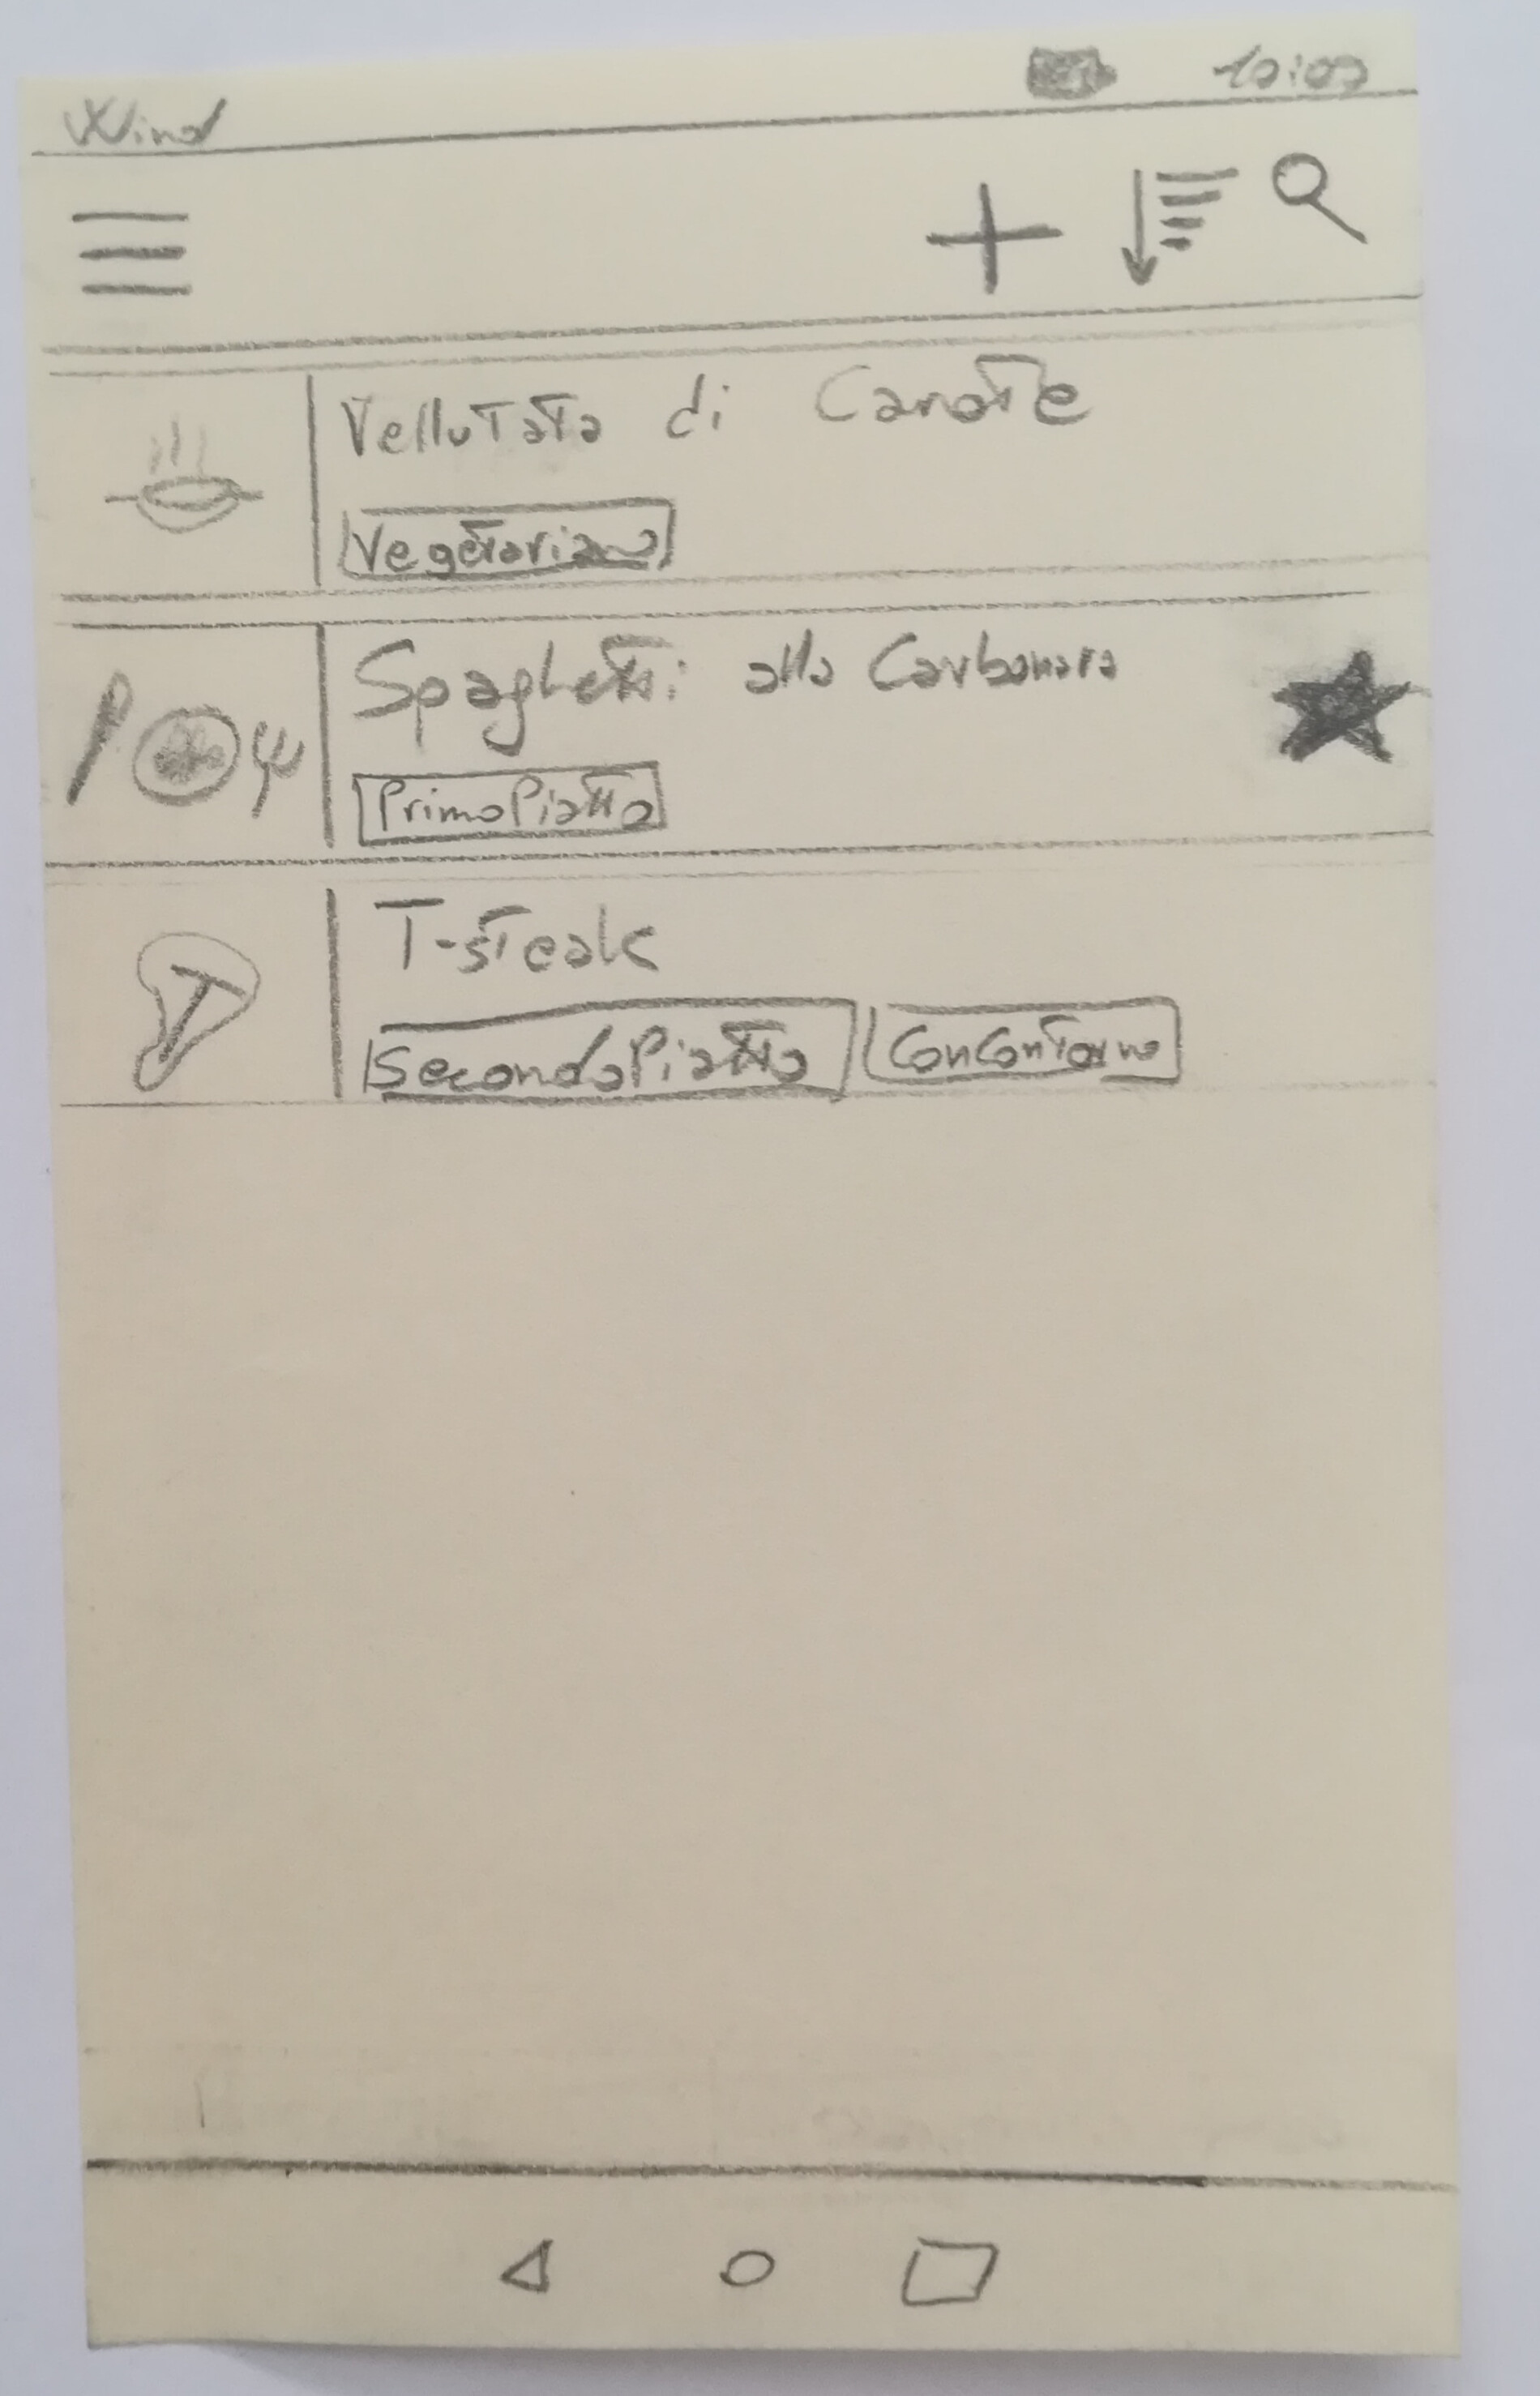
\includegraphics[width=0.6\textwidth]{prototipo1/main_ricette_lista_tags}
%    \caption{Primo storyboard}
%    \label{fig:roa}
%  \end{center}
%\end{figure}







\section{Secondo Assignment}
In questo \textit{assignment} vengono illustrato il processo di creazione e raffinamento del prototipo per l'applicazione Ricettavola.
Ciascun prototipo è stato testato su una decina di persone in una fascia d'età tra i 20 e i 30 anni.
Gli intervistati hanno anche valutato alcuni design alternativi.


\subsection{Primo Prototipo Low-Fidelity}

\subsubsection{Descrizione del Design}

In figura~\ref{fig:p1_main} a sinistra è riportata la schermata principale dell'applicazione.
Le ricette vengono mostrate in una lista, ogni elemento mostra l'immagine associata alla ricetta, il suo titolo, eventuali etichette (ad esempio primo piatto, secondo piatto, vegetariano, contorno, \dots ) e se la ricetta appartiene ai preferiti.
I tasti in alto a sinistra indicano la possibilità di aggiungere una nuova ricetta, ordinare le ricette oppure cercarne una.
Nella schermata affianco si è valutata la possibilità di spostare il tasto di creazione di una nuova ricetta in un \textit{floating action button} posizionato in basso a destra.

\begin{figure}[ht]
  \begin{center}
    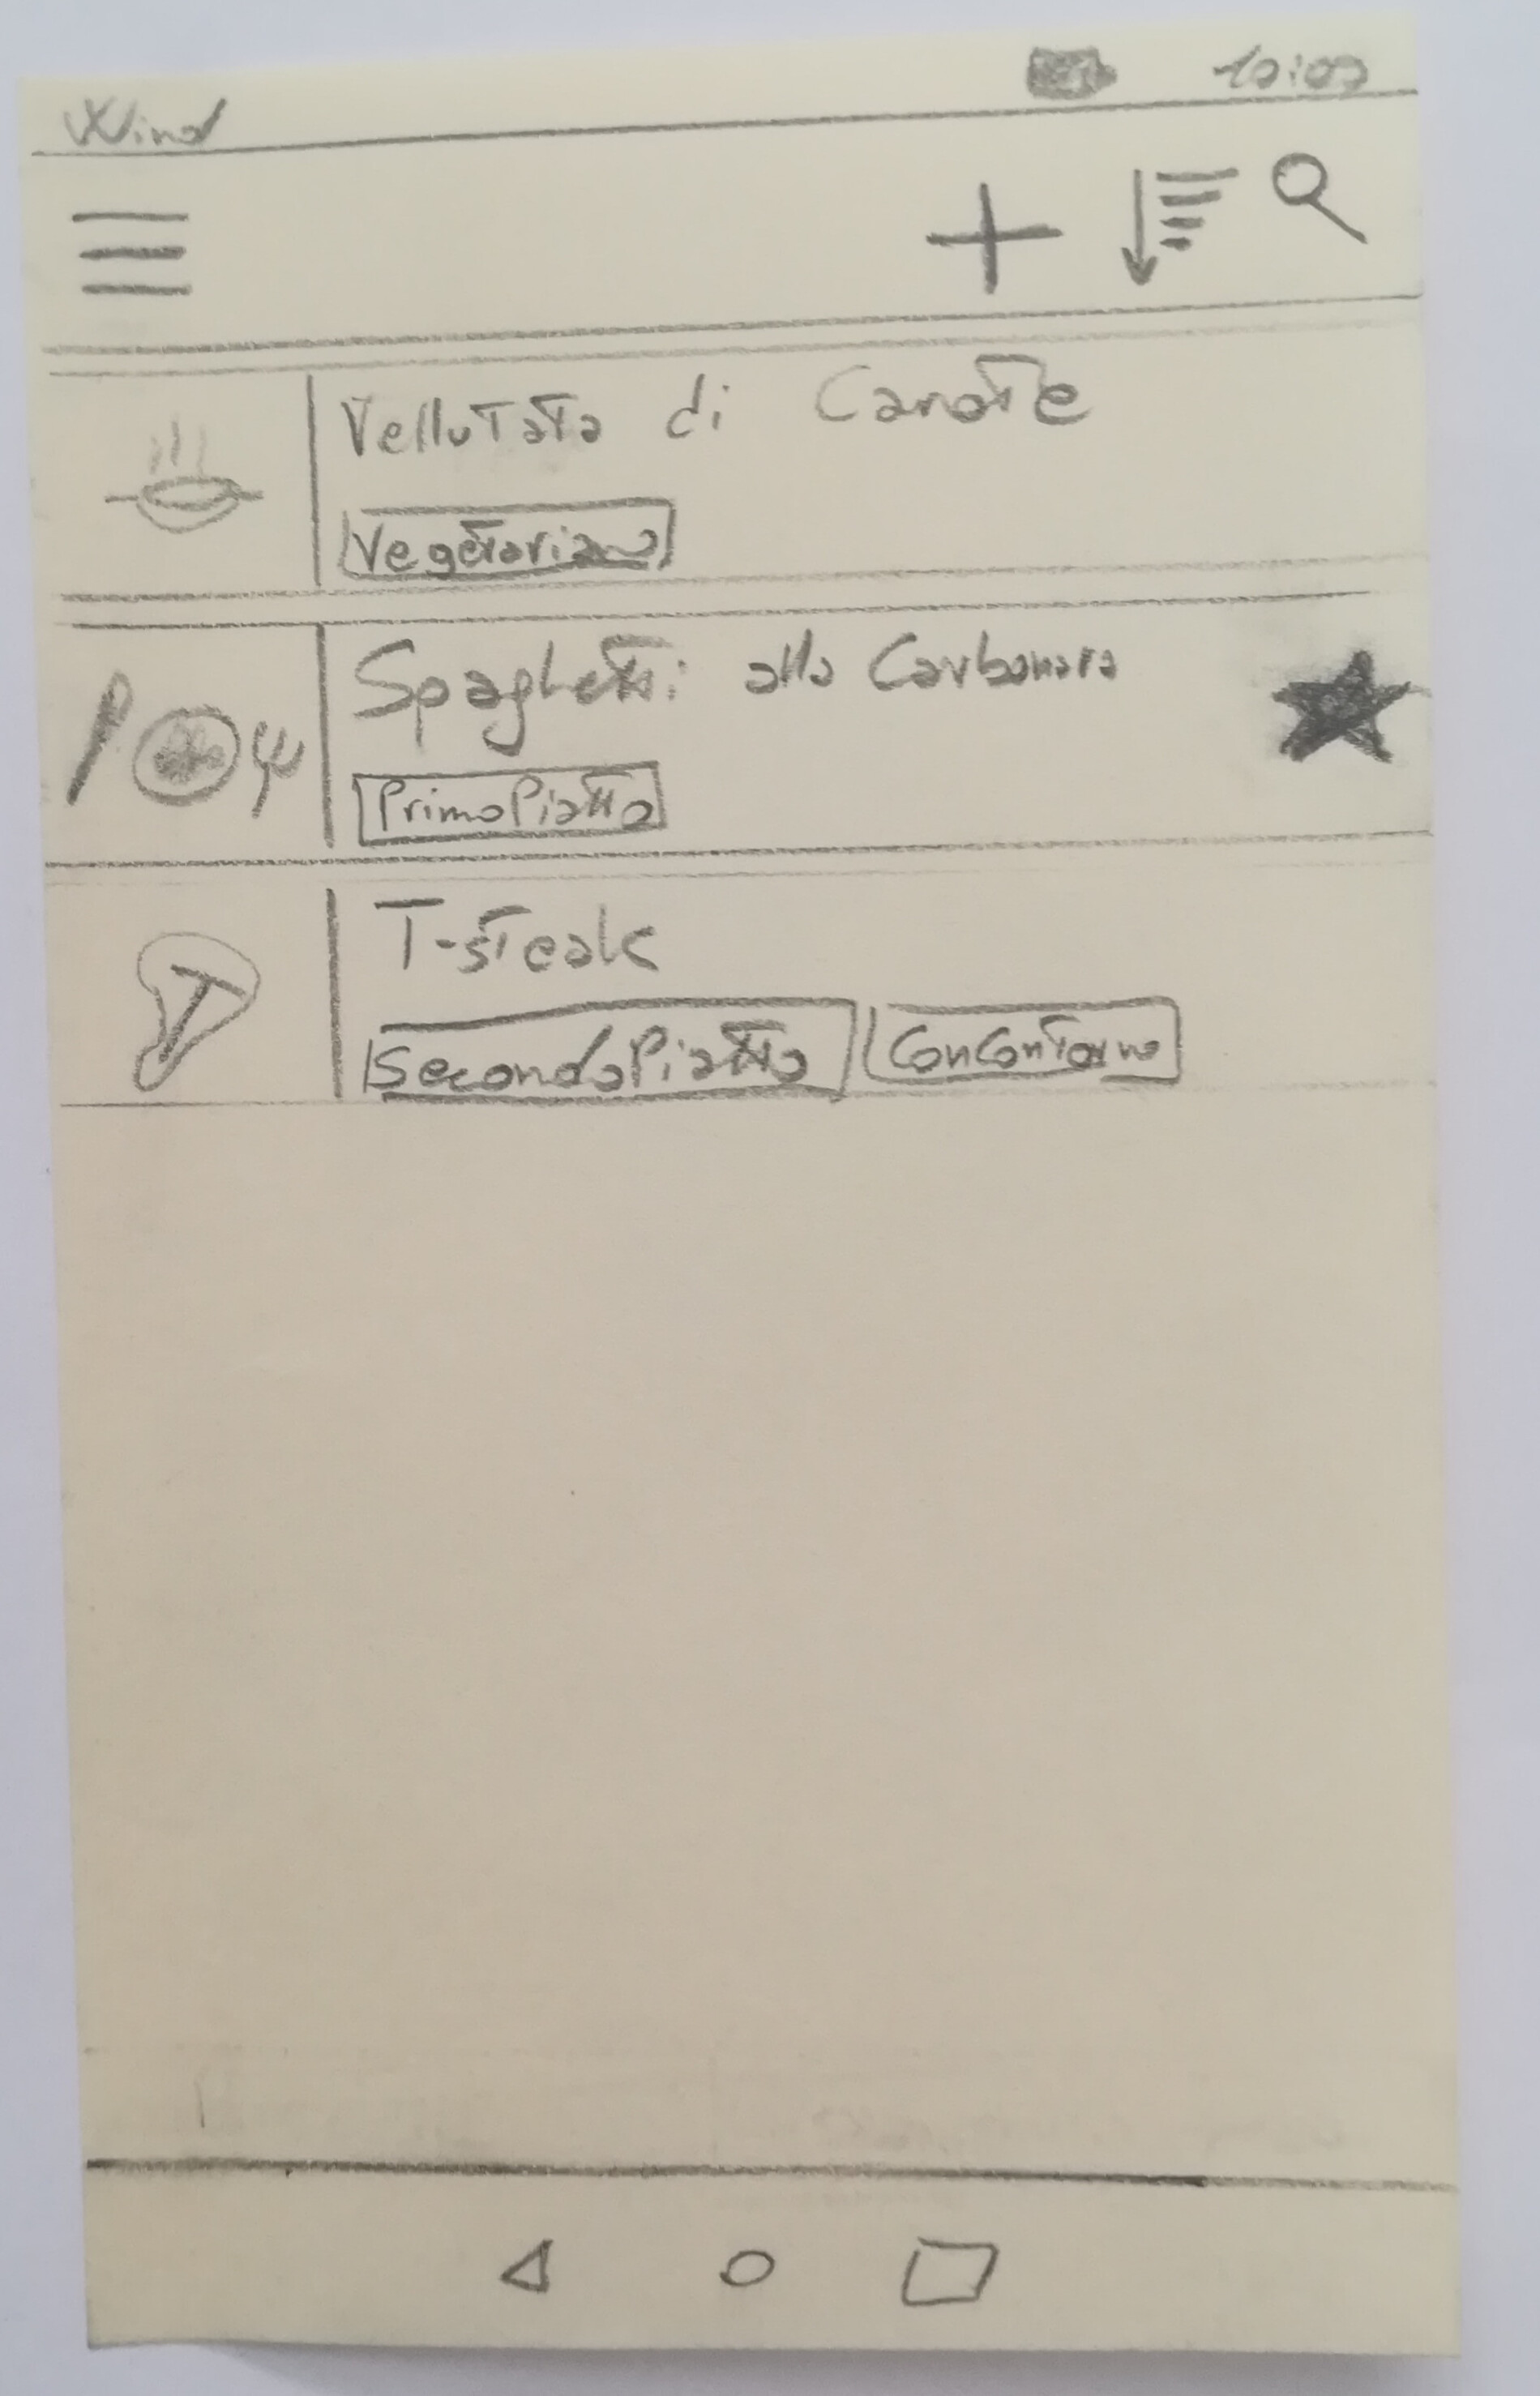
\includegraphics[width=0.45\textwidth]{prototipo1/main_ricette_lista_tags}
    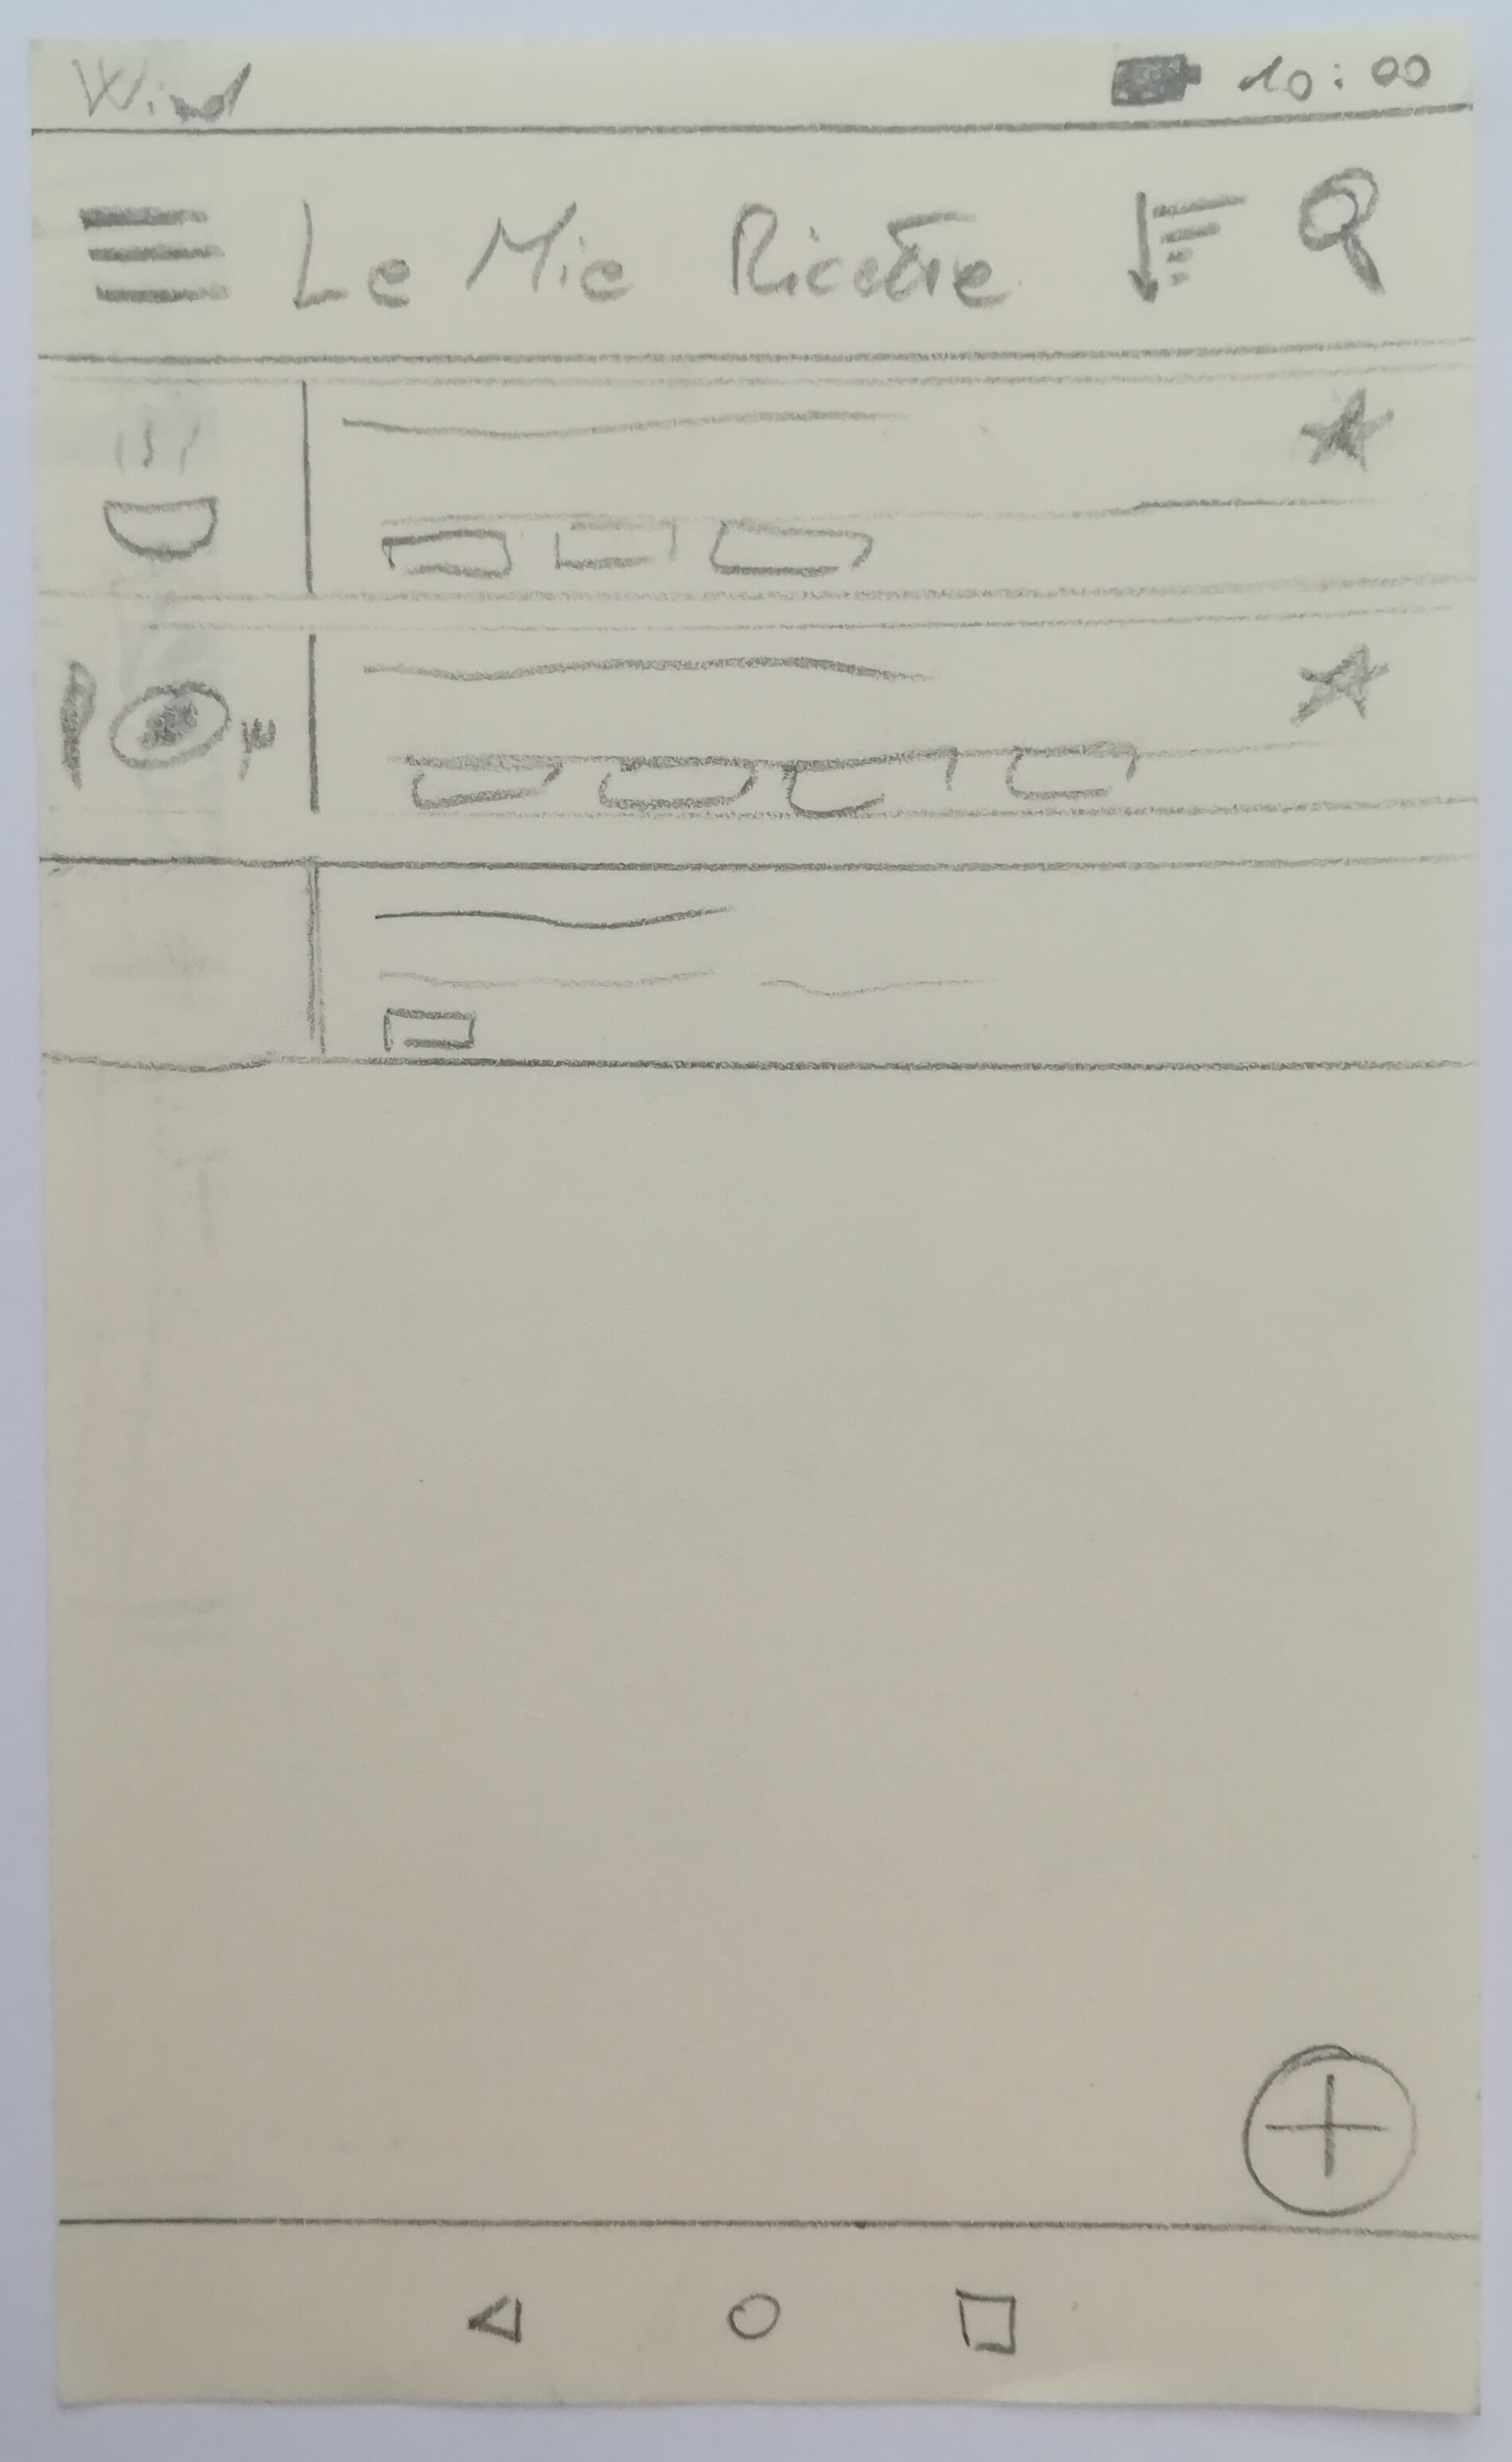
\includegraphics[width=0.43\textwidth]{prototipo1/main_ricette_lista_tags_fab}
    \caption{Schermata principale}
    \label{fig:p1_main}
  \end{center}
\end{figure}

\clearpage
Premendo il tasto in alto a sinistra si apre una TODO laterale, riportata a sinistra in figura \ref{fig:p1_lista_spesa}.
Qui è possibile effettuare varie operazioni, tra cui visualizzare la lista della spesa.
Quest'ultima è divisa in due sezioni in modo che risulti chiaro quali sono gli ingredienti ancora da comprare e quali invece sono già stati acquistati.
Si fa notare che non è presente alcun tasto per l'aggiunta degli ingredienti.
Infatti lo scopo di questa lista è limitarsi a tener traccia degli ingredienti delle ricette che si vogliono cucinare.

\begin{figure}[ht]
  \begin{center}
    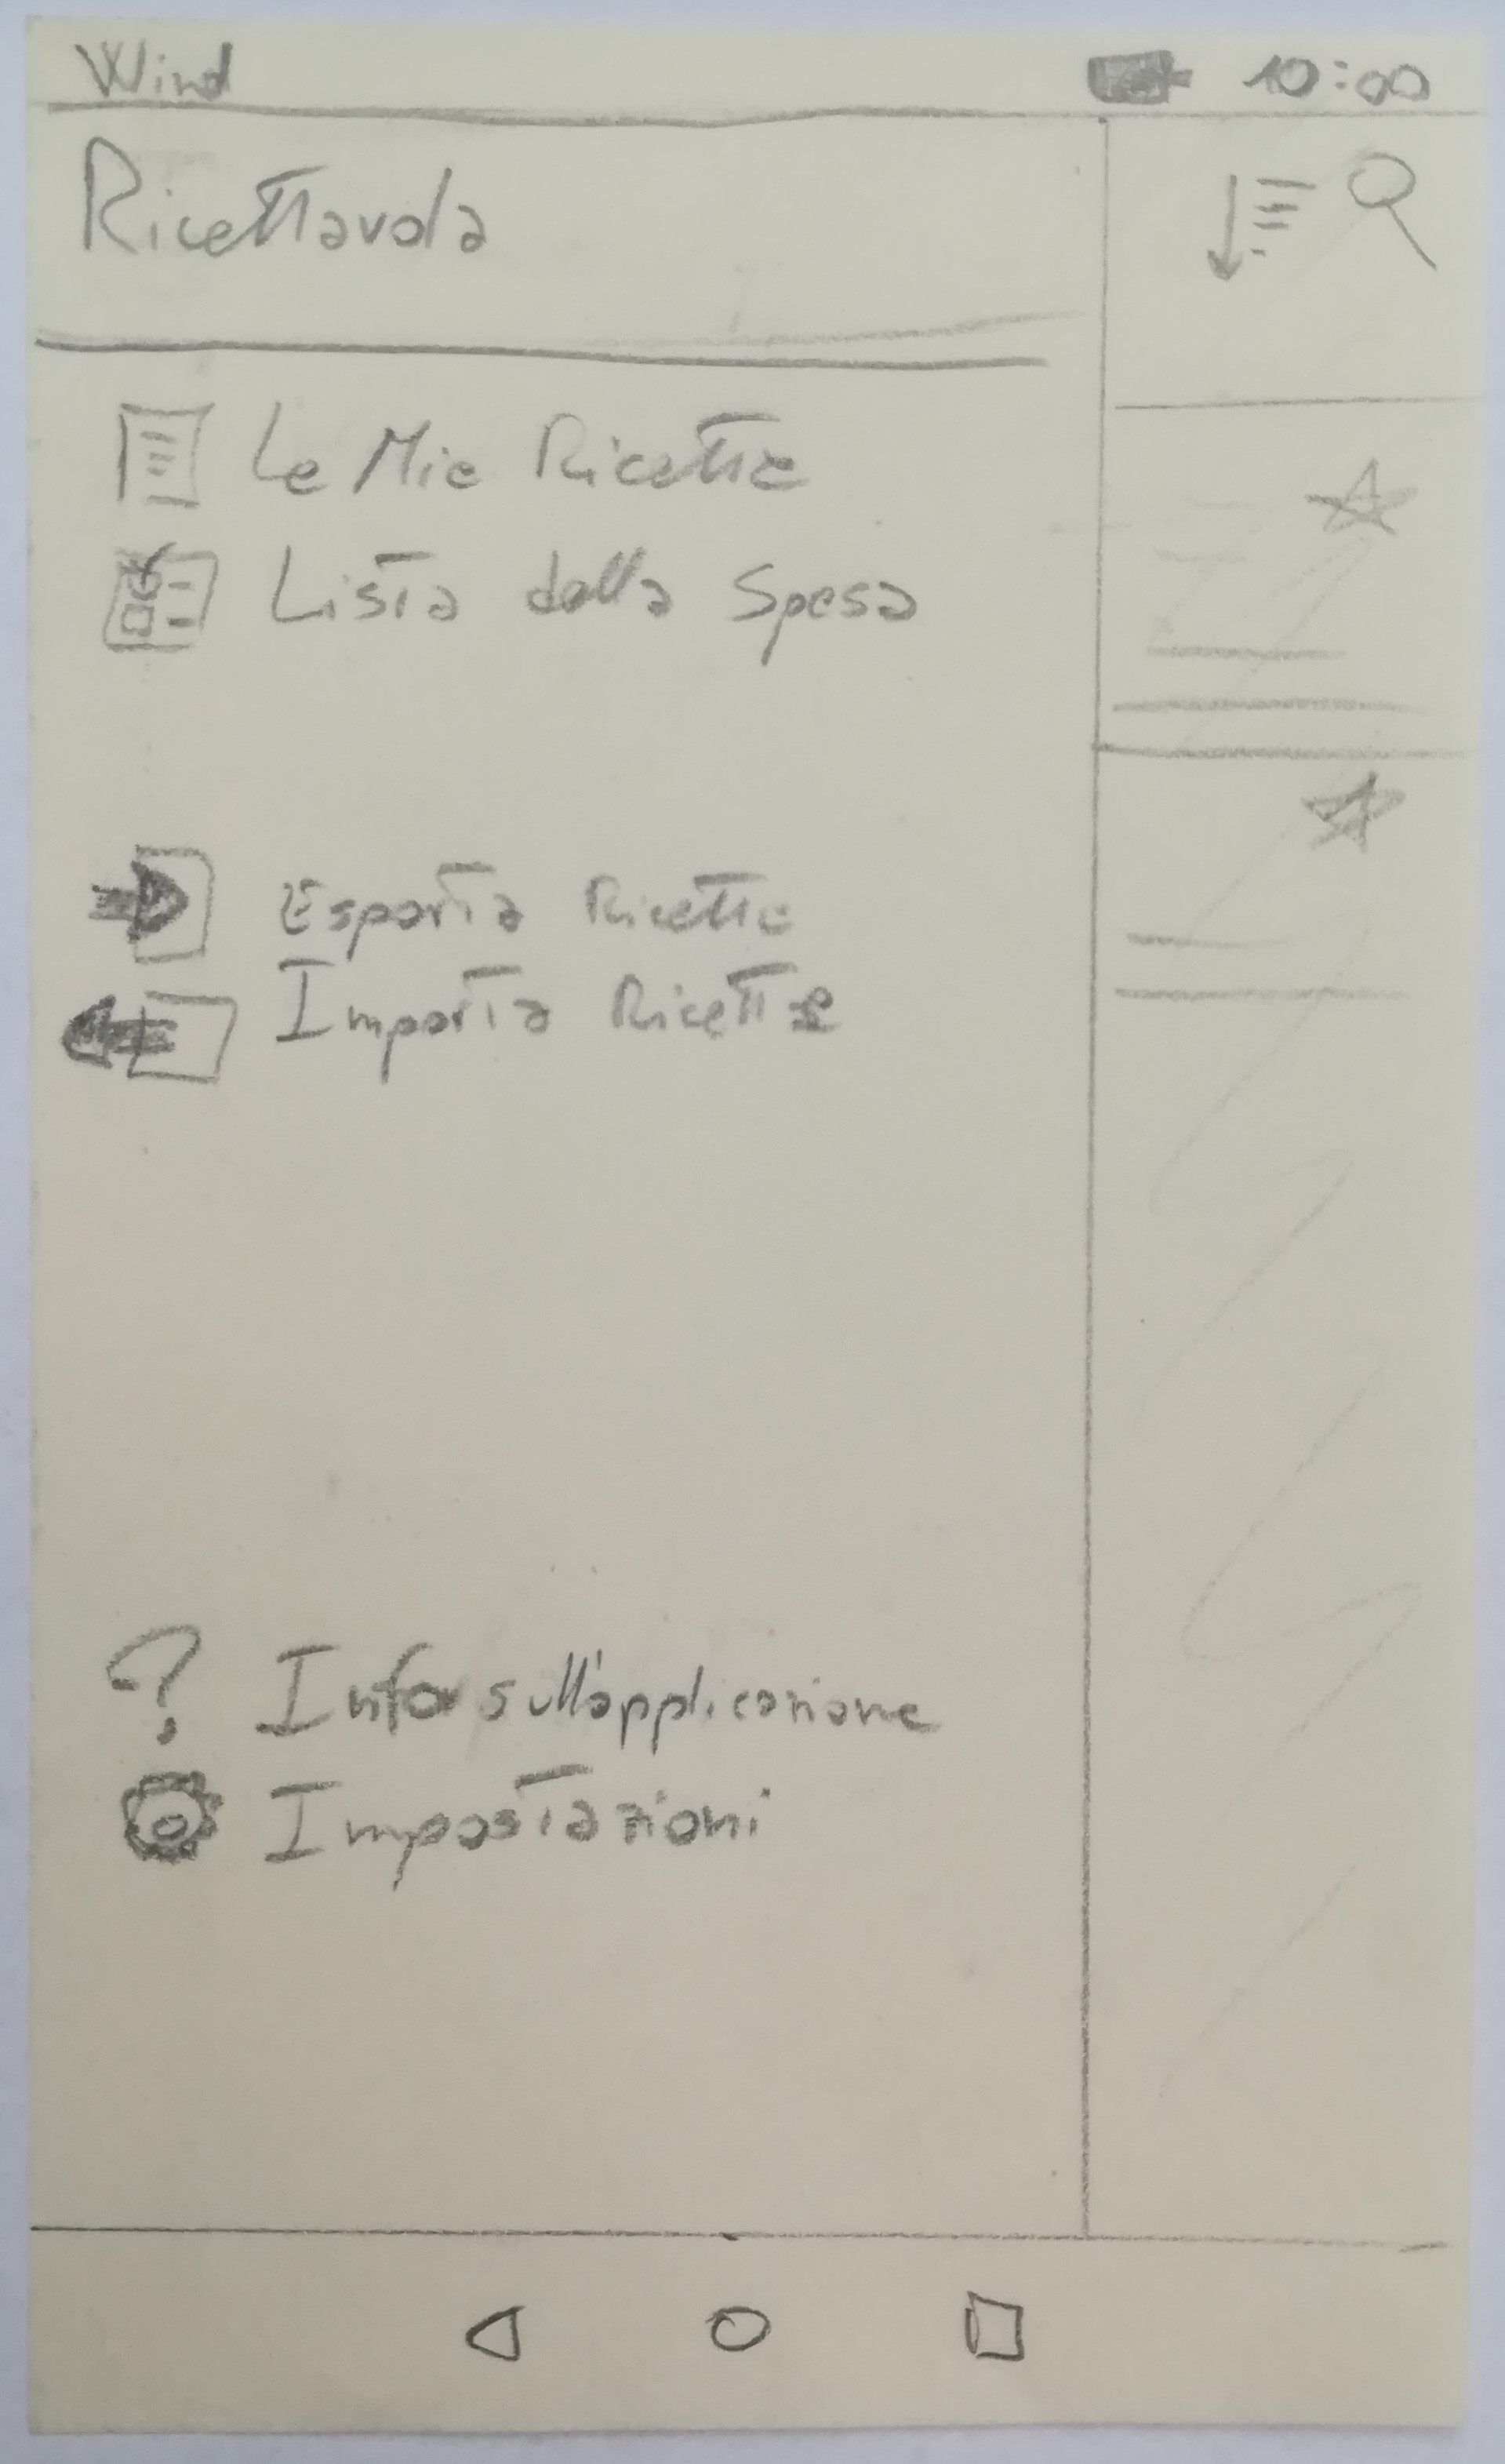
\includegraphics[width=0.47\textwidth]{prototipo1/tab_laterale}
    \includegraphics[width=0.49\textwidth]{prototipo1/main_lista_della_spesa}
    \caption{Da sinistra a destra: TODO laterale, la lista della spesa}
    \label{fig:p1_lista_spesa}
  \end{center}
\end{figure}


\clearpage
Dalla attività principale, premendo una ricetta, si passa alle prima schermata in figura \ref{fig:p1_ricetta}.
Nel toolbar sono presenti alcune azioni comuni, come modificare o condividere la ricetta, e ovviamente la possibilità di tornare alla schermata precedetene.
I tre pallini in fondo al toolbar nascondono un menù a tendina in cui dovrà comparire la voce "Aggiungi nella lista della spesa".
Poco sotto il toolbar sono presenti tre tab: Riepilogo, Ingredienti, Preparazione.
La prima linguetta è selezionata, infatti si possono osservare le principali informazioni della ricetta selezionata.
Premendo su una linguetta o con un'azione di \textit{swipe} si può passare alle altre schermate.
La seconda immagine mostra tutti gli ingredienti necessari, inoltre offre la possibilità di incrementare automaticamente la quantità di ingredienti in funzione del numero di persone.
L'ultima schermata illustra i passaggi numerati della ricetta.
Il tasto "Cuciamo!" in fondo allo schermo permette di avviare la modalità assistente per questa ricetta.

\begin{figure}[ht]
  \begin{center}
    \includegraphics[width=0.325\textwidth]{prototipo1/ricetta_riepilogo}
    \includegraphics[width=0.325\textwidth]{prototipo1/ricetta_ingredienti}
    \includegraphics[width=0.325\textwidth]{prototipo1/ricetta_preparazione}
    \caption{Da sinistra a destra: riepilogo, ingredienti, preparazione}
    \label{fig:p1_ricetta}
  \end{center}
\end{figure}

Prima di spiegare quali sono le schermate della modalità assistente, si vuole fare una parentesi sulla modalità di modifica di una ricetta.
In figura \ref{fig:p1_edit_ricetta} si possono osservare come le schermate di figura \ref{fig:p1_ricetta} vengono modificate quando viene premuto il tasto a forma di matita.
Ovviamente anche la toolbar deve essere modificato perché essere possibile salvare la ricetta dopo averla modificata, ma non è accettabile che si voglia condividere una ricetta in fase di modifica.
La prima schermata permette di modificare il tempo di preparazione attraverso delle freccette.
Notare che ogni campo contenente testo diventa modificabile.
La possibilità di poter arrangiare l'ordine di ingredienti e passaggi della preparazione è indicato dalle tre barre orizzontali vicine ad ogni elemento delle liste.

Si fa presente che alla creazione di una nuova ricetta si viene rimandati all'equivalente vuoto delle schermate in figura \ref{fig:p1_edit_ricetta}.
Ogni campo verrà compilato da suggerimenti così da guidare l'utente nella compilazione.

\begin{figure}[ht]
  \begin{center}
    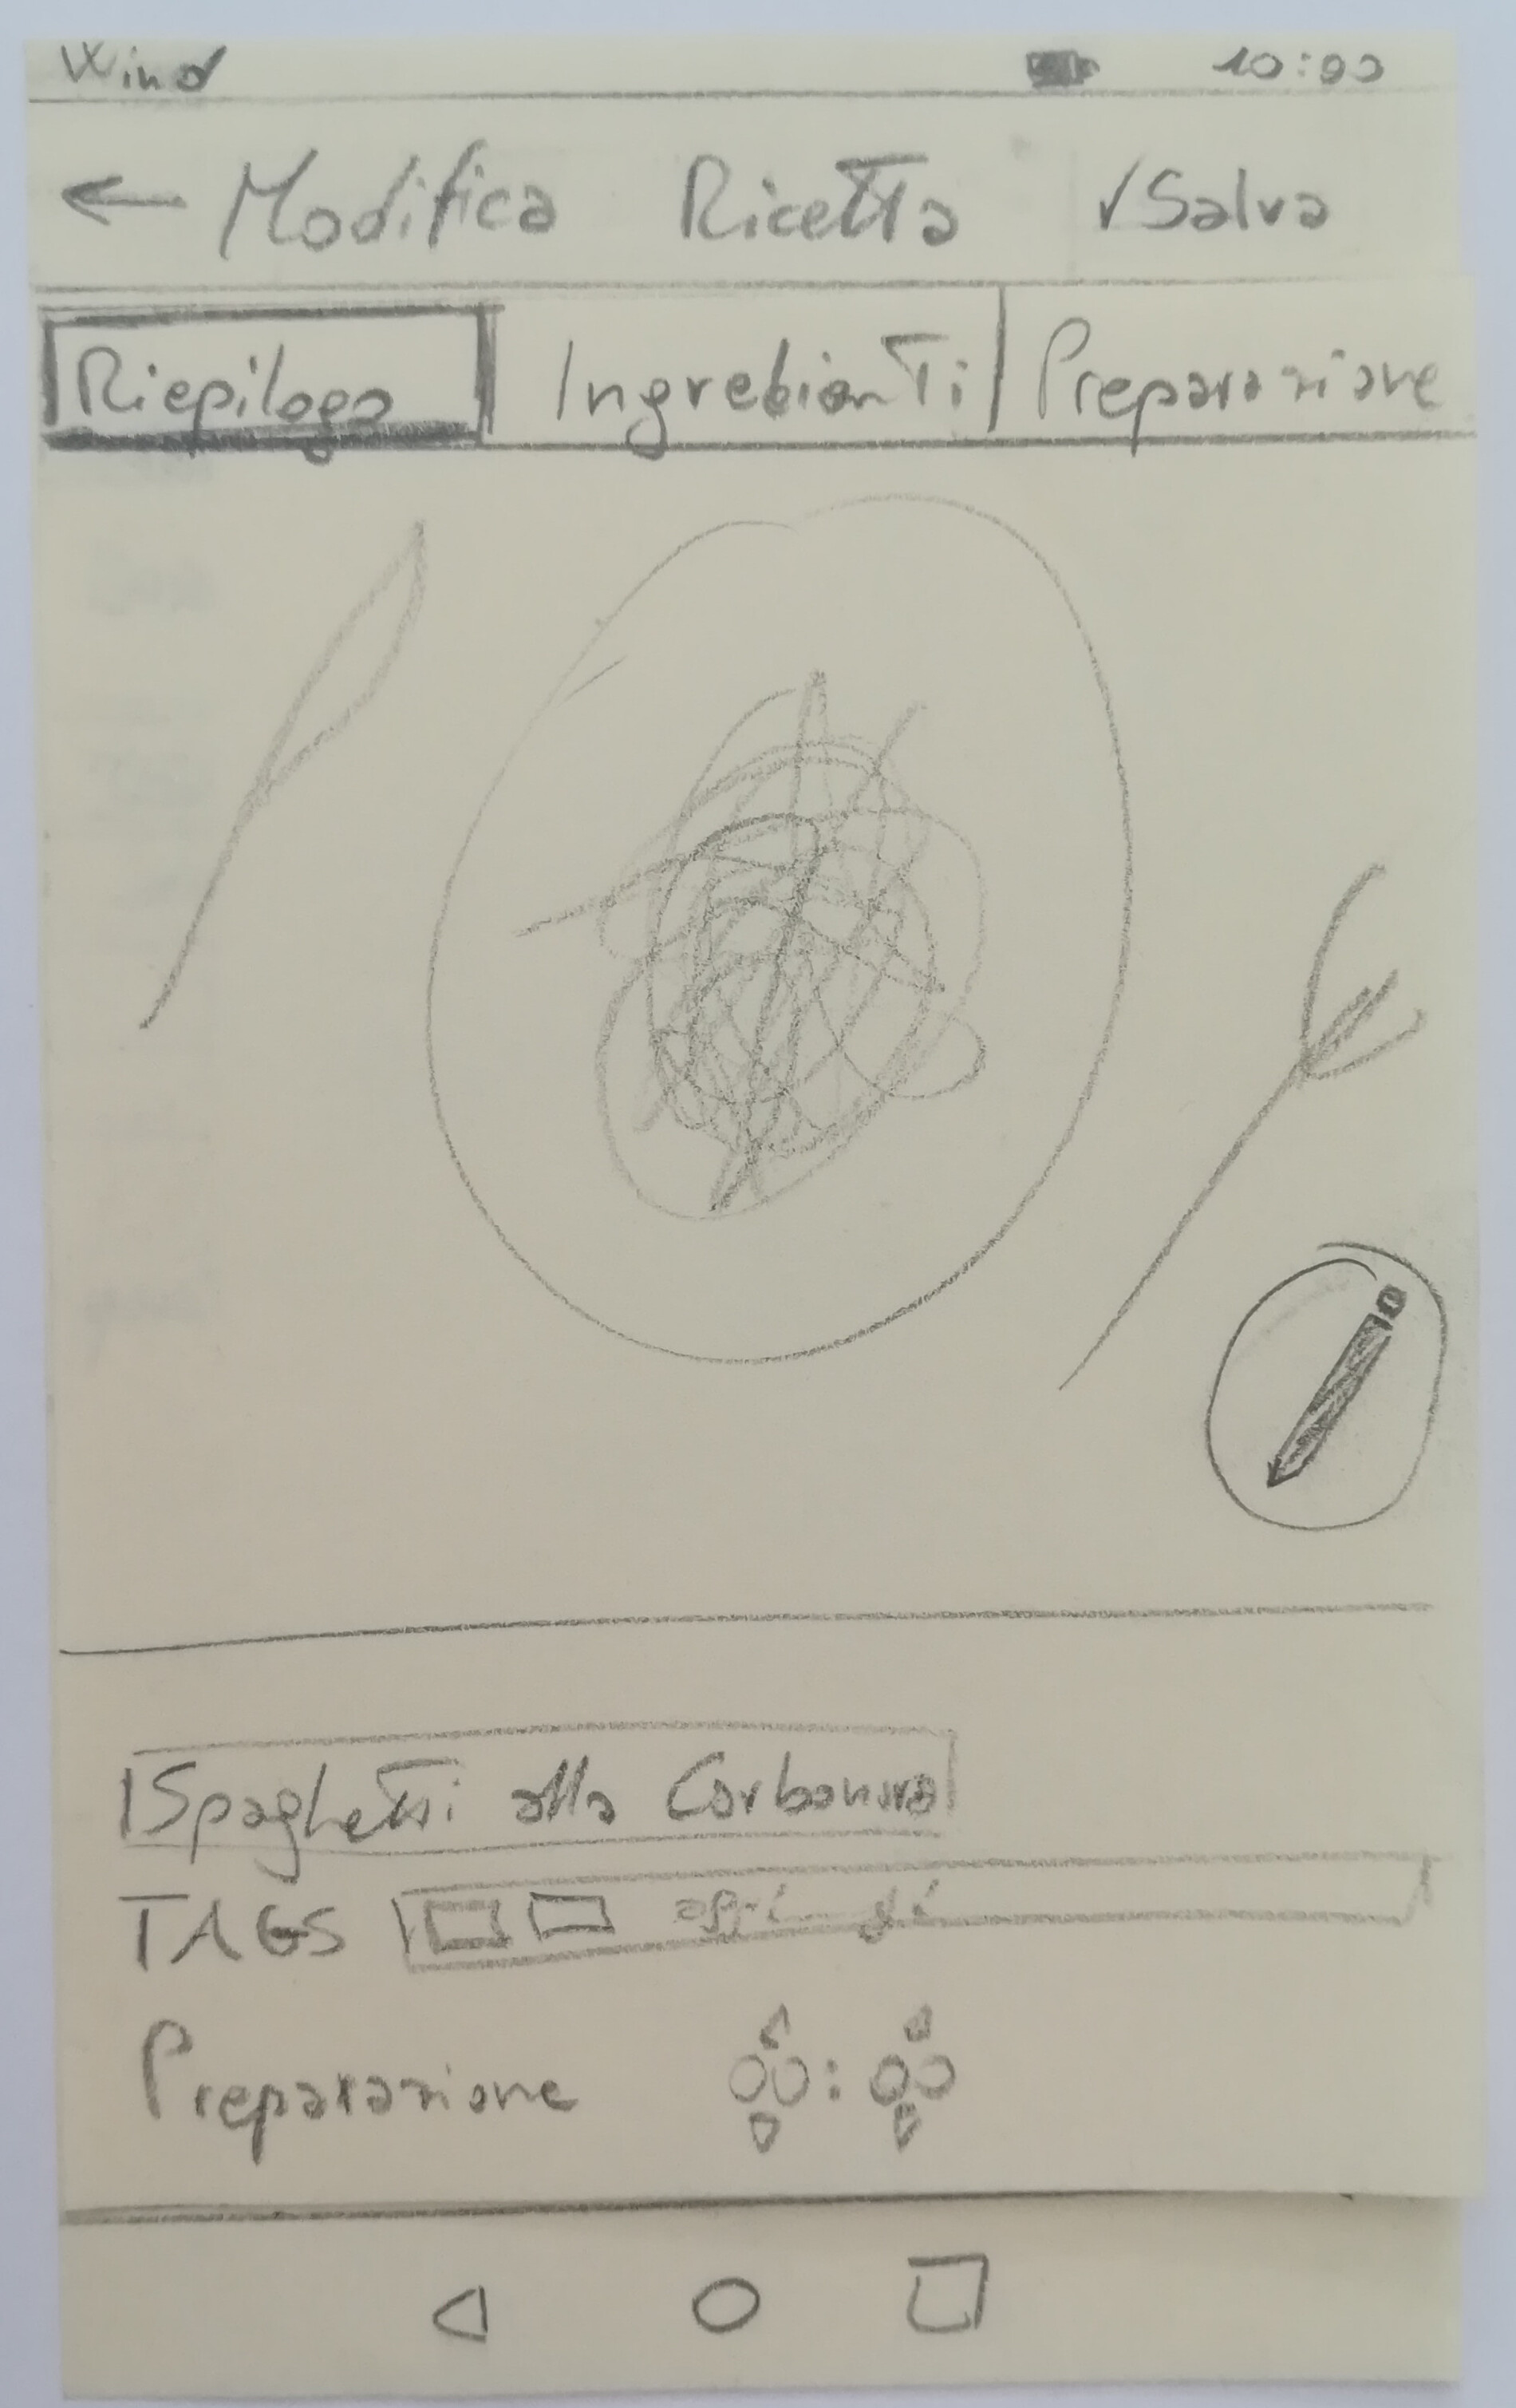
\includegraphics[width=0.325\textwidth]{prototipo1/edit_ricetta_riepilogo}
    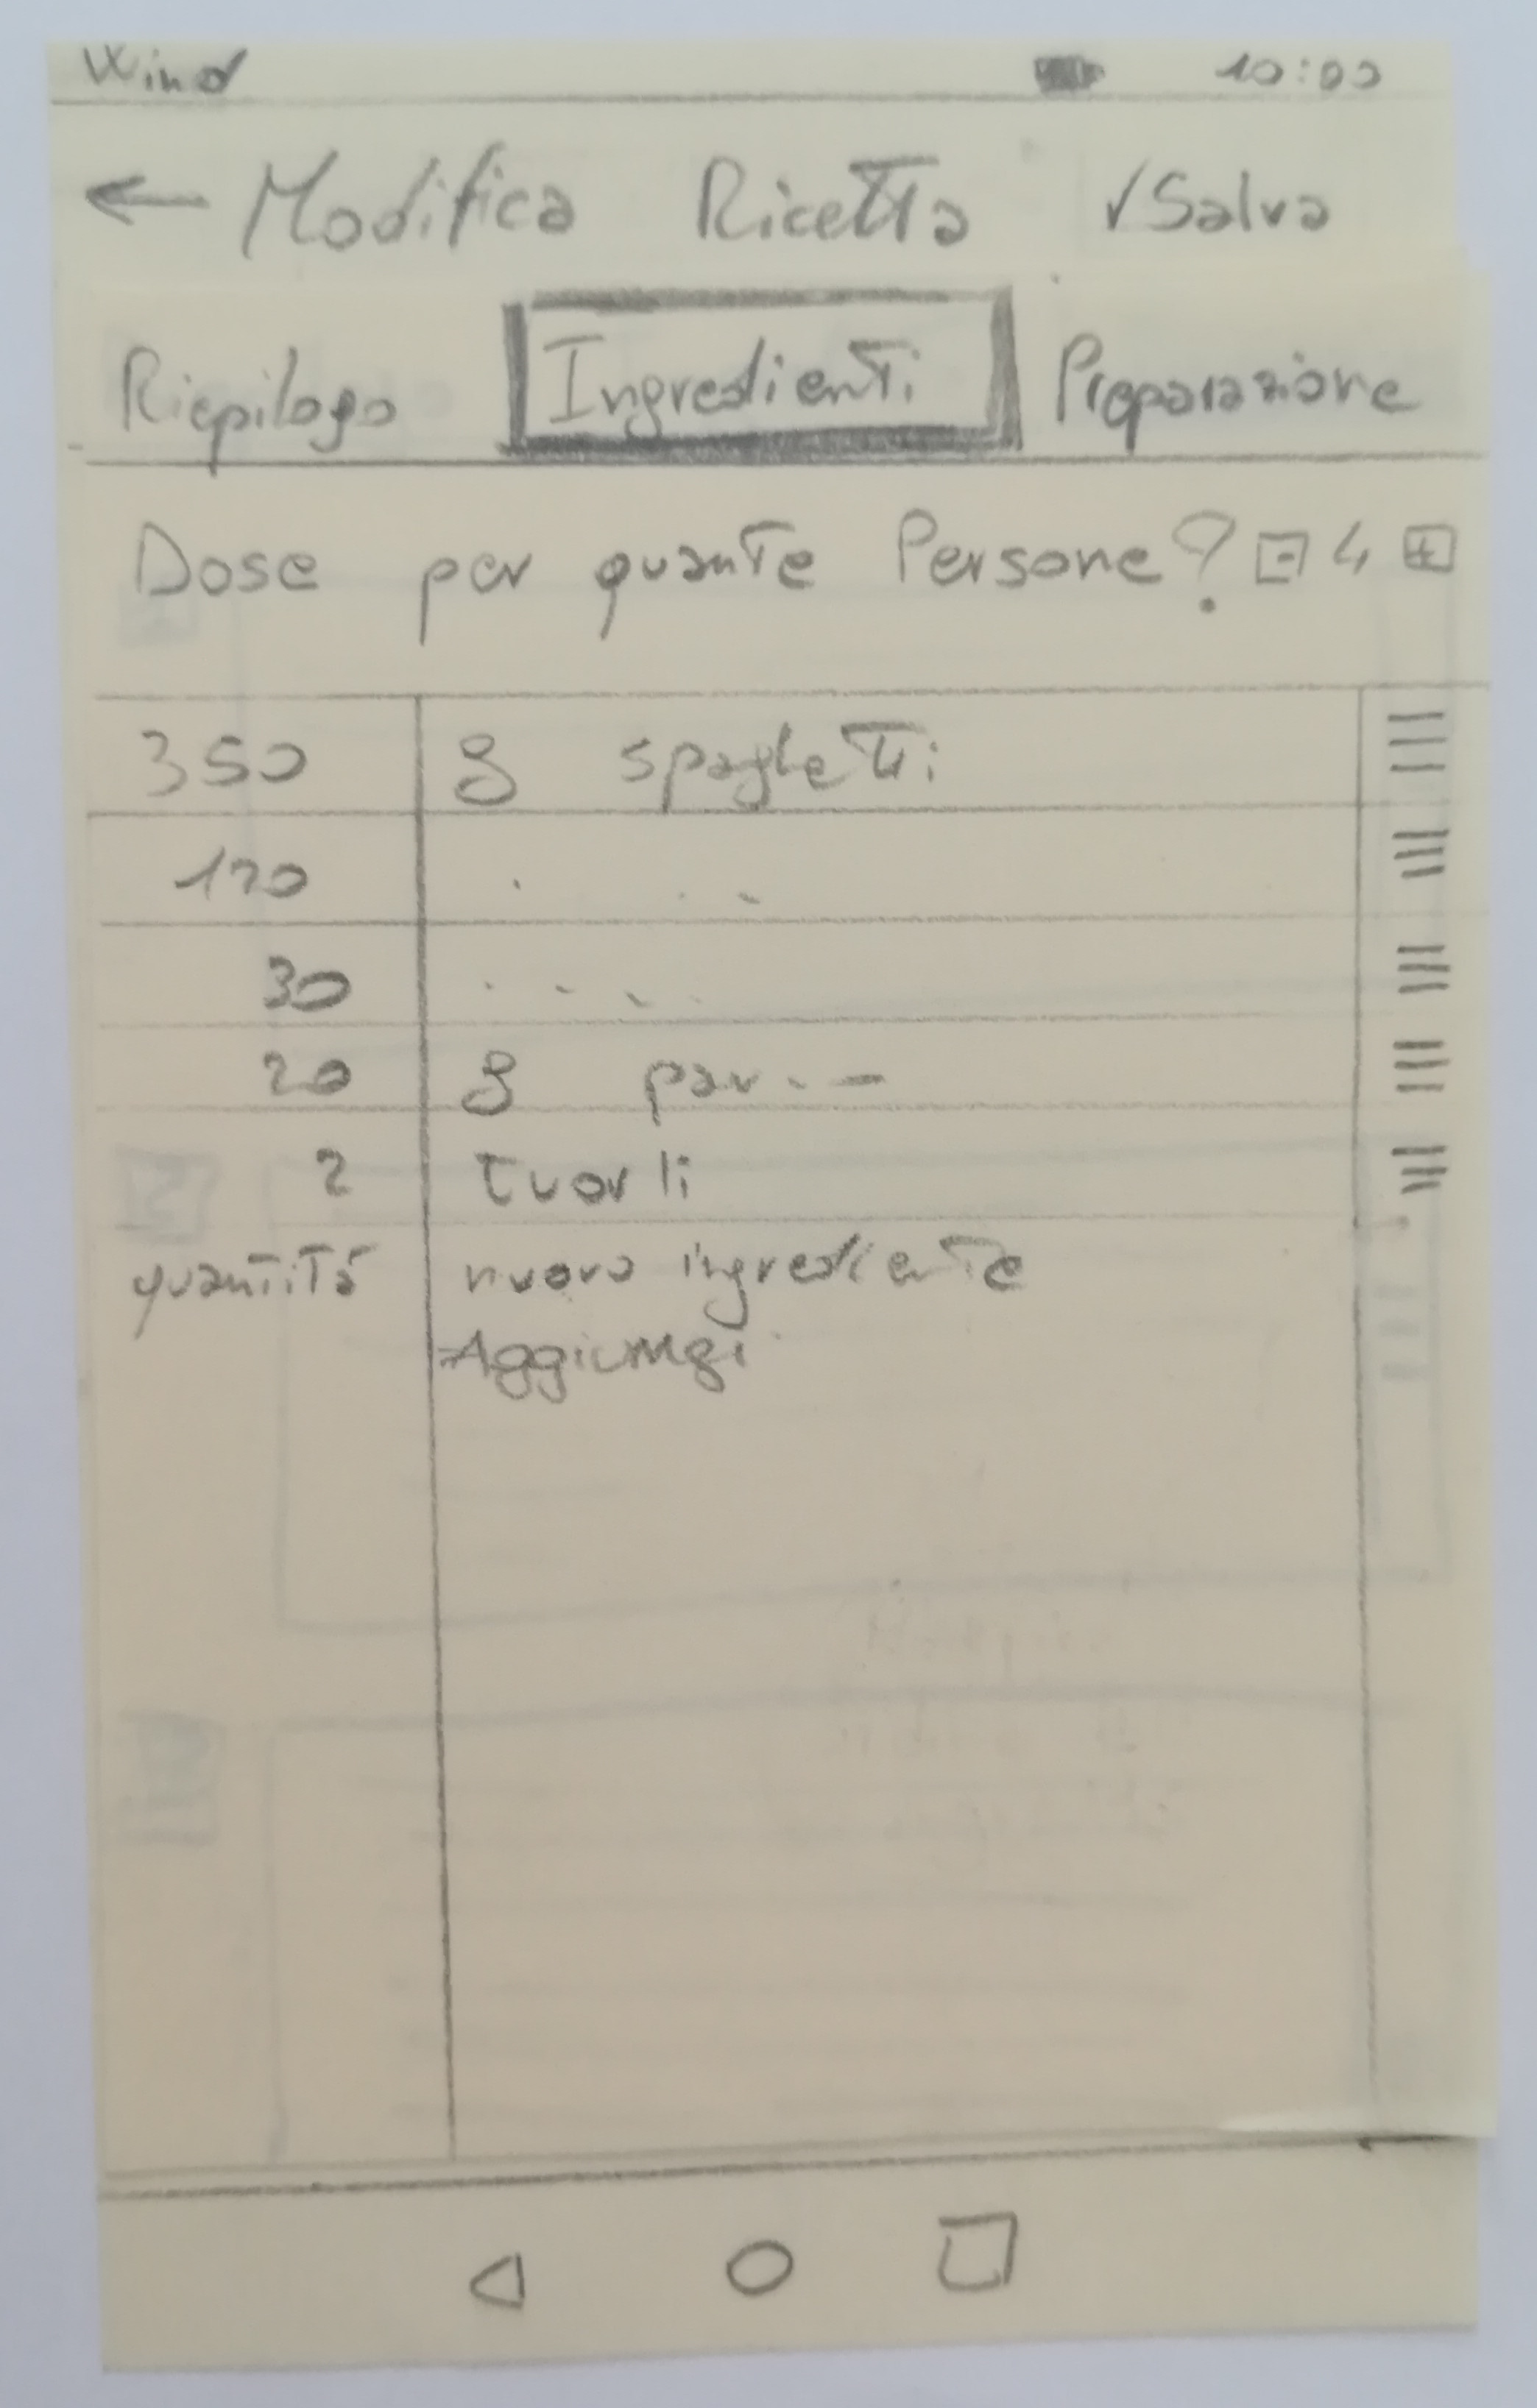
\includegraphics[width=0.325\textwidth]{prototipo1/edit_ricetta_ingredienti}
    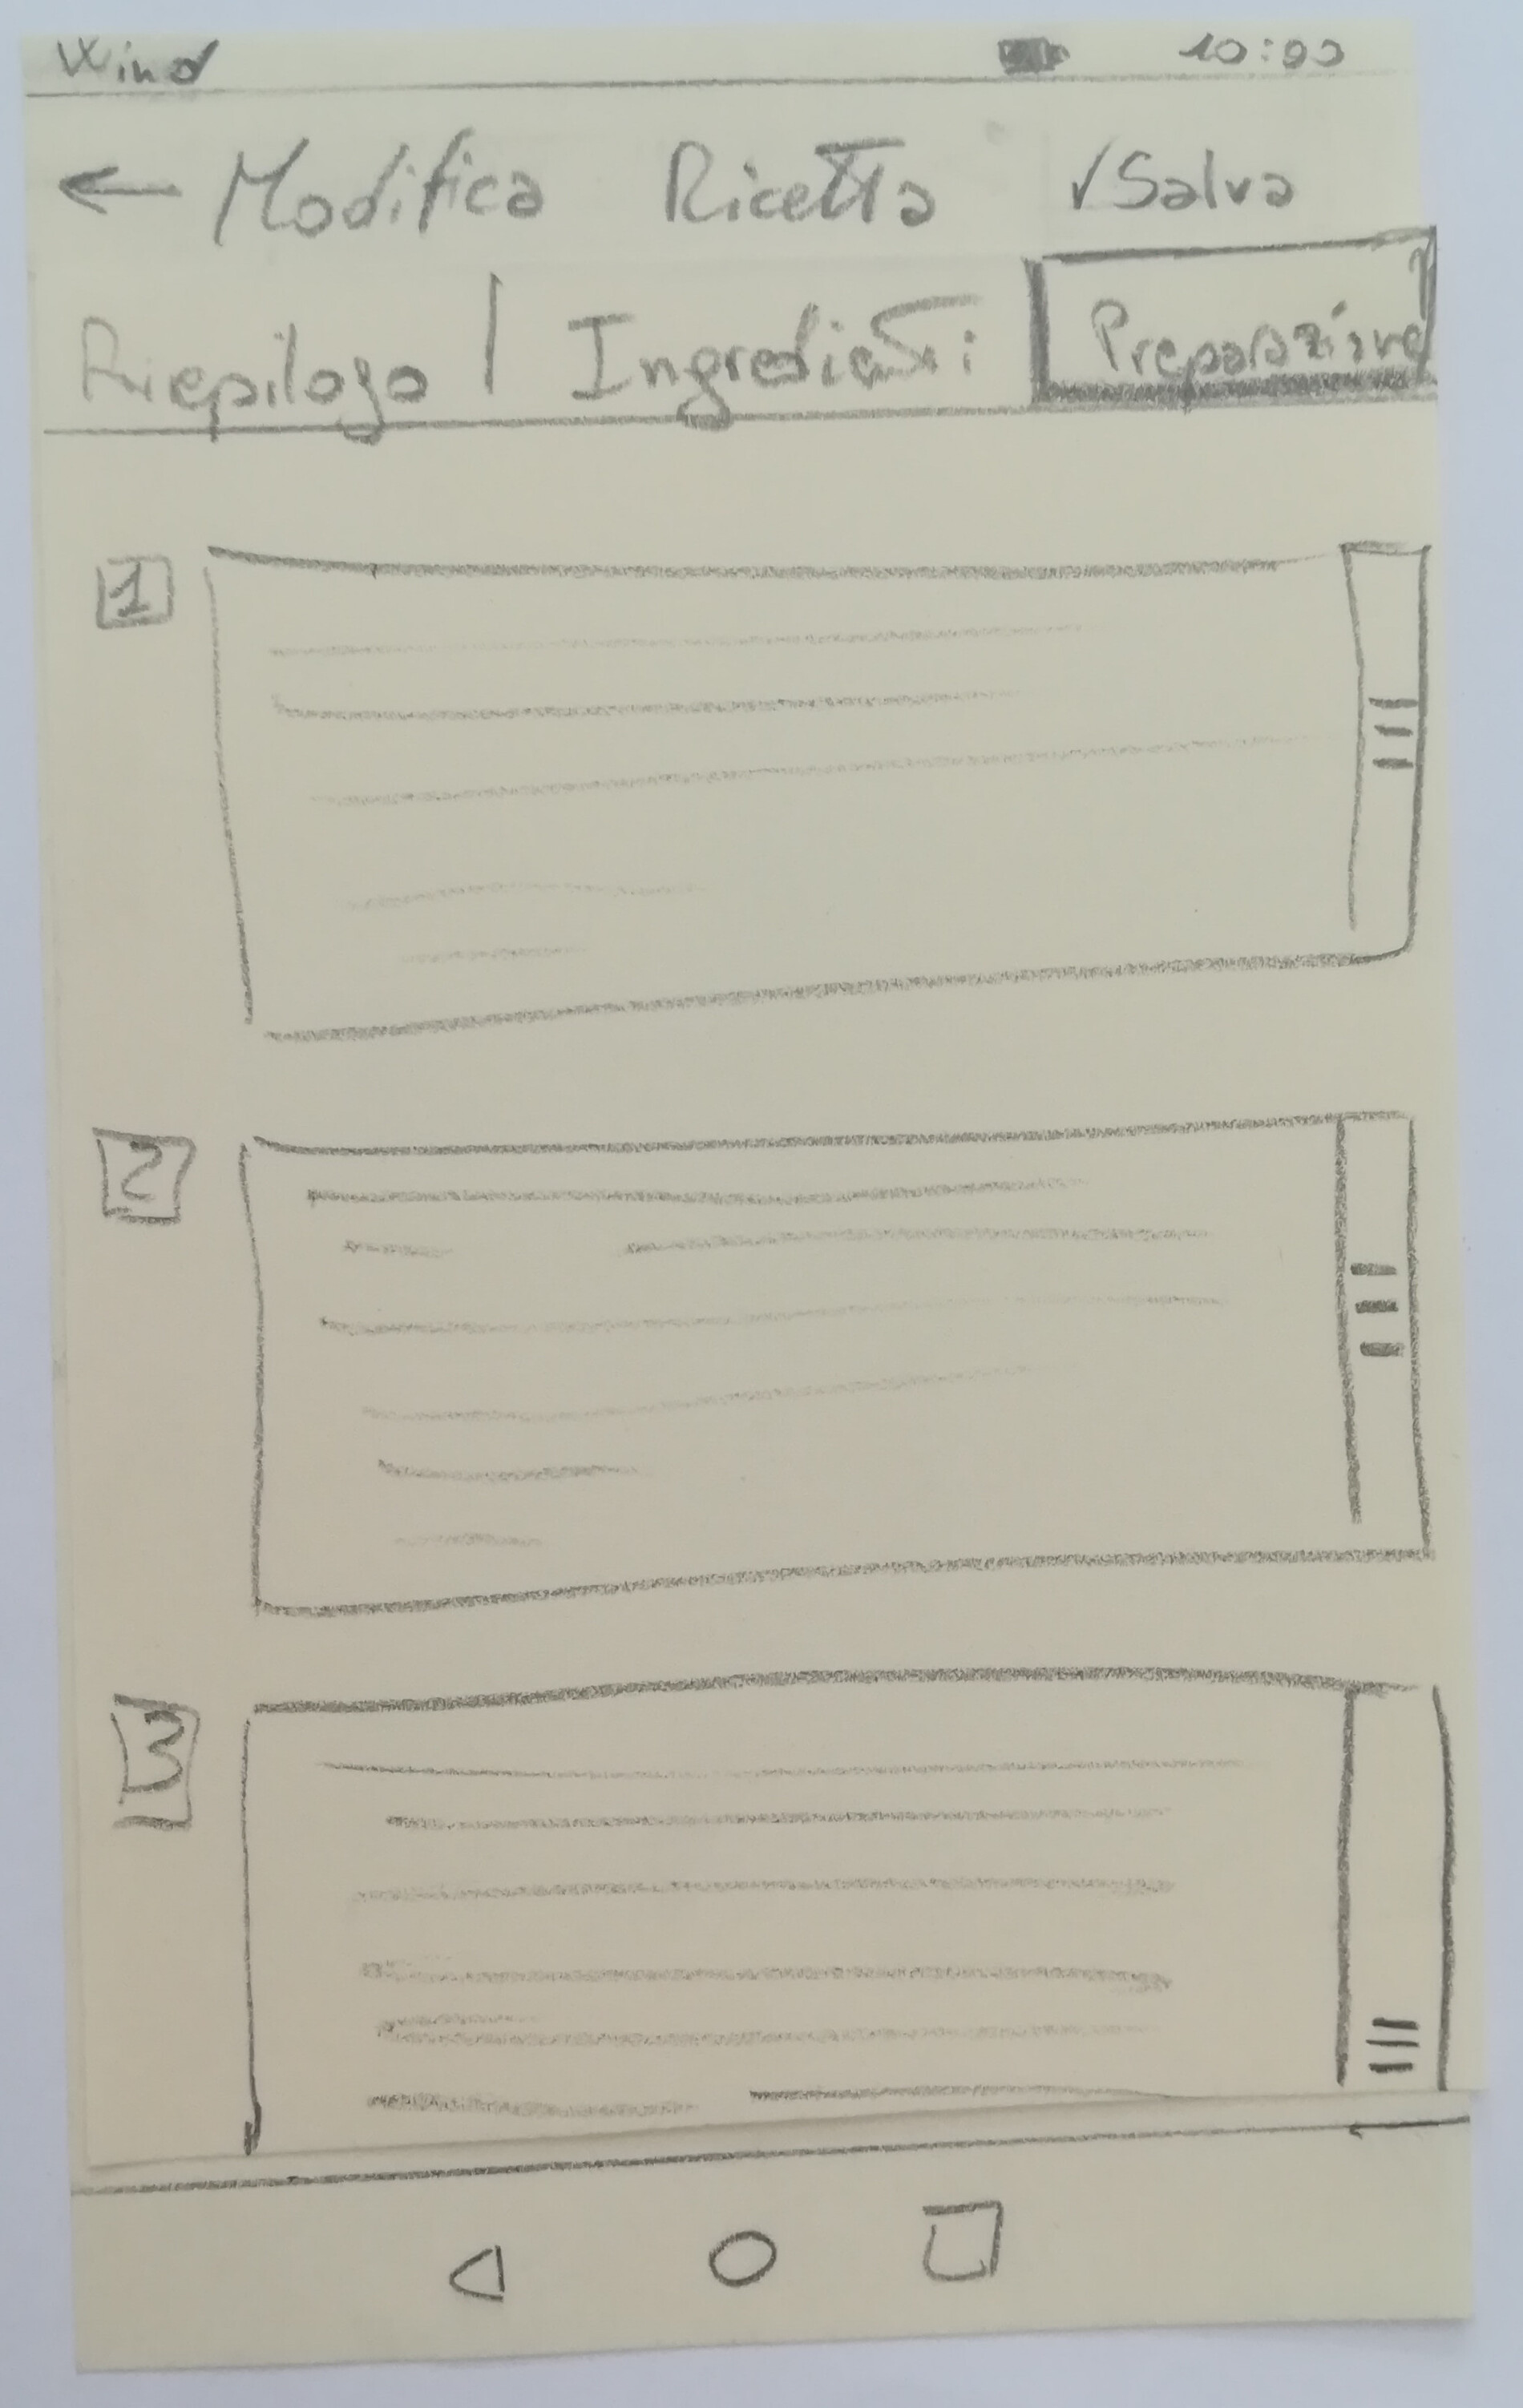
\includegraphics[width=0.325\textwidth]{prototipo1/edit_ricetta_preparazione}
    \caption{Da sinistra a destra: riepilogo, ingredienti, preparazione}
    \label{fig:p1_edit_ricetta}
  \end{center}
\end{figure}


In figura \ref{fig:p1_cuciniamo} sono mostrate tre versioni differenti della schermata assistente.
Innanzitutto si fa notare che le queste schermate sono pensate per essere usate esclusivamente in modalità \textit{landscape}.
Questa scelta è stata fatta per tentare di massimizzare la dimensione del testo nella schermata, così che fosse facilmente leggibile anche da una certa distanza.
Un altro punto in comune fra le schermate è quello di presentare due tasti ben visibili per procedere al prossimo passo oppure per rileggere quelli già effettuati.
Il criterio con cui questi tasti sono stati creati è quello di permettere all'utente di spostarsi tra i passaggi della ricetta sporcando soltanto due zone dello schermo.
Si può ipotizzare infatti che chi cucina abbia le mani bagnate o sporche di pasta, con i due tasti appena descritti si vuole minimizzare l'area toccata con le dita.
Ogni schermata presenta in alto il numero dello step corrente.
È sembrato utile integrare questa schermata con un timer, così da averlo sempre a portata di mano.

La seconda schermata ha una funzione in più rispetto alle altre perché permette di osservare, nel riquadro sotto a quello dell'orologio, gli ingredienti della ricetta.

\clearpage
\begin{figure}[ht]
  \begin{center}
    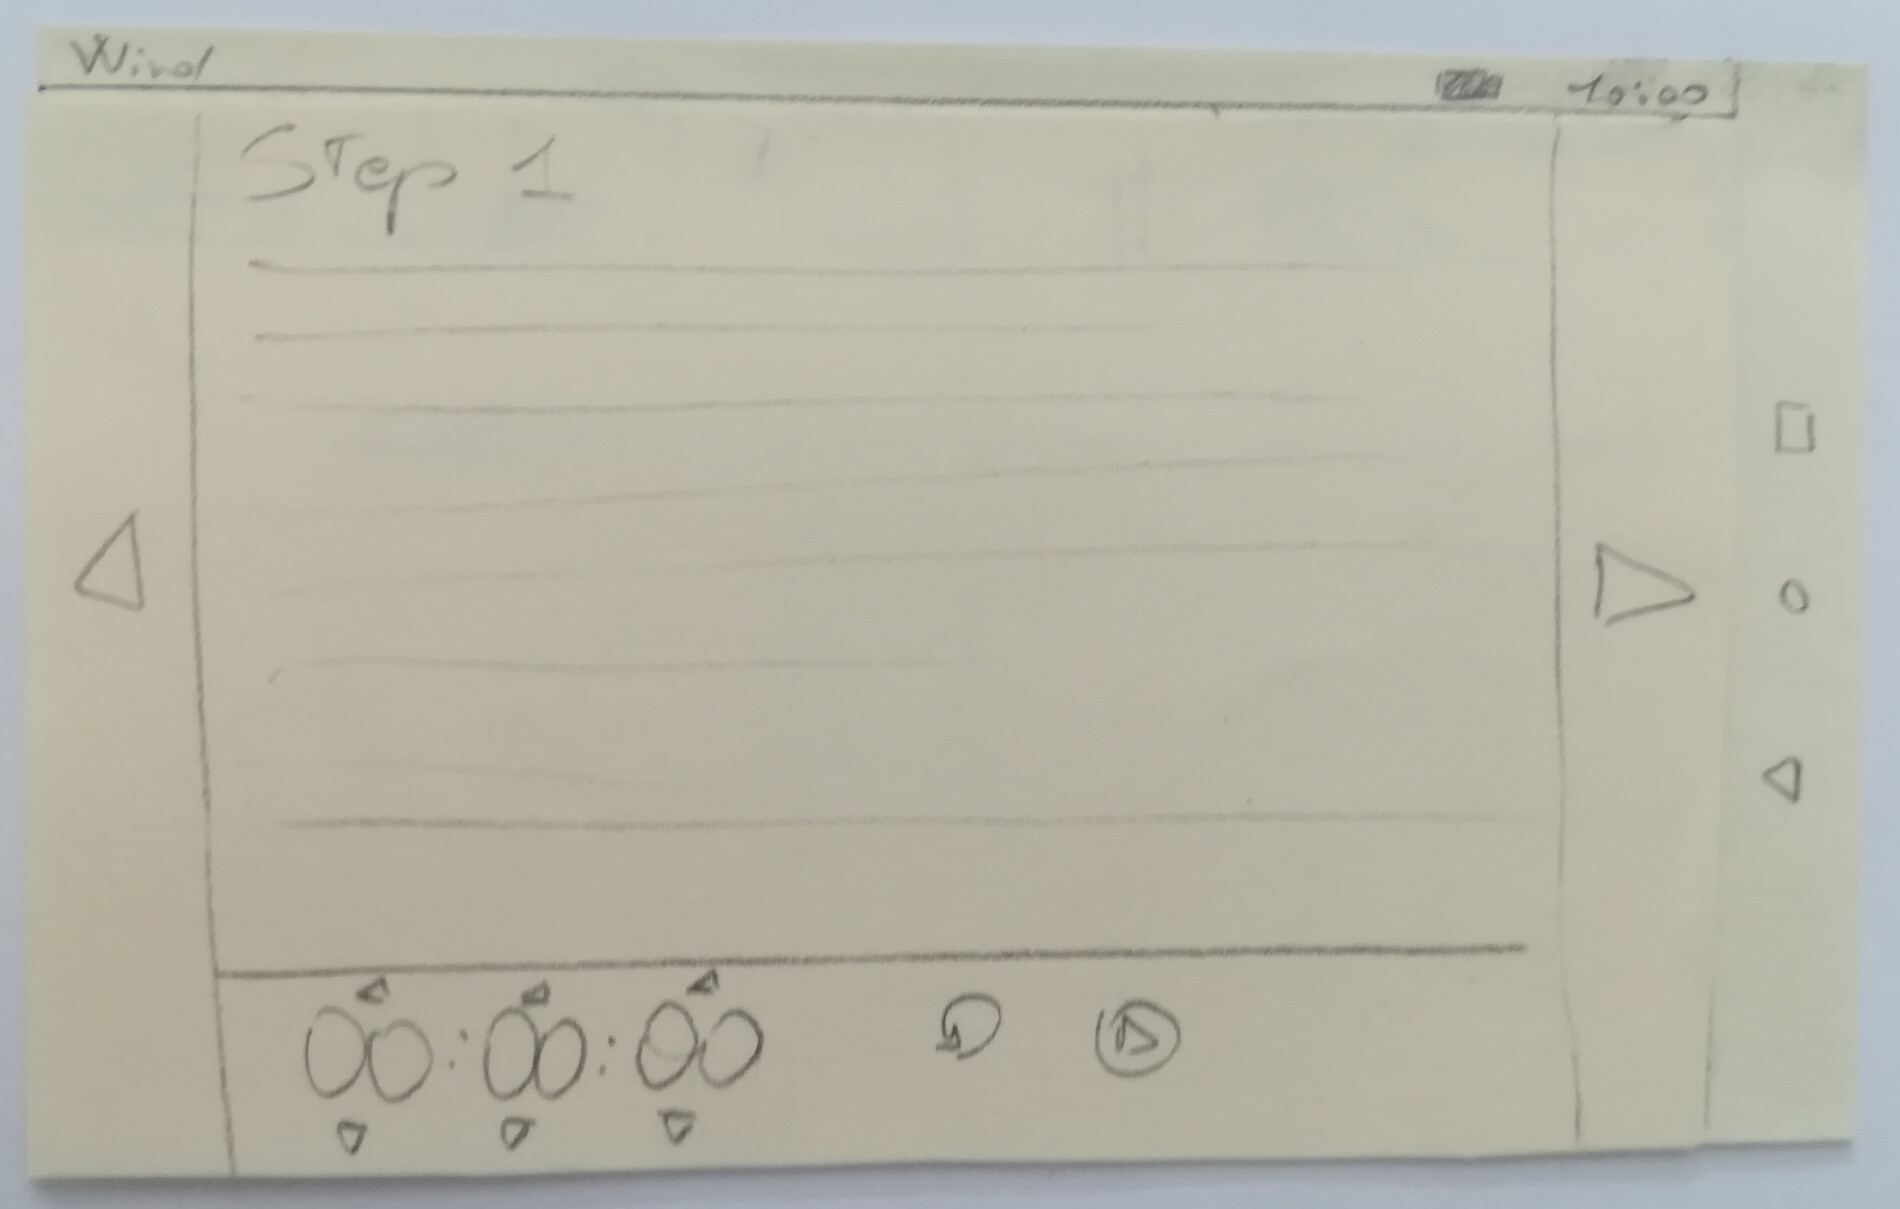
\includegraphics[width=0.78\textwidth]{prototipo1/cuciamo_a}
    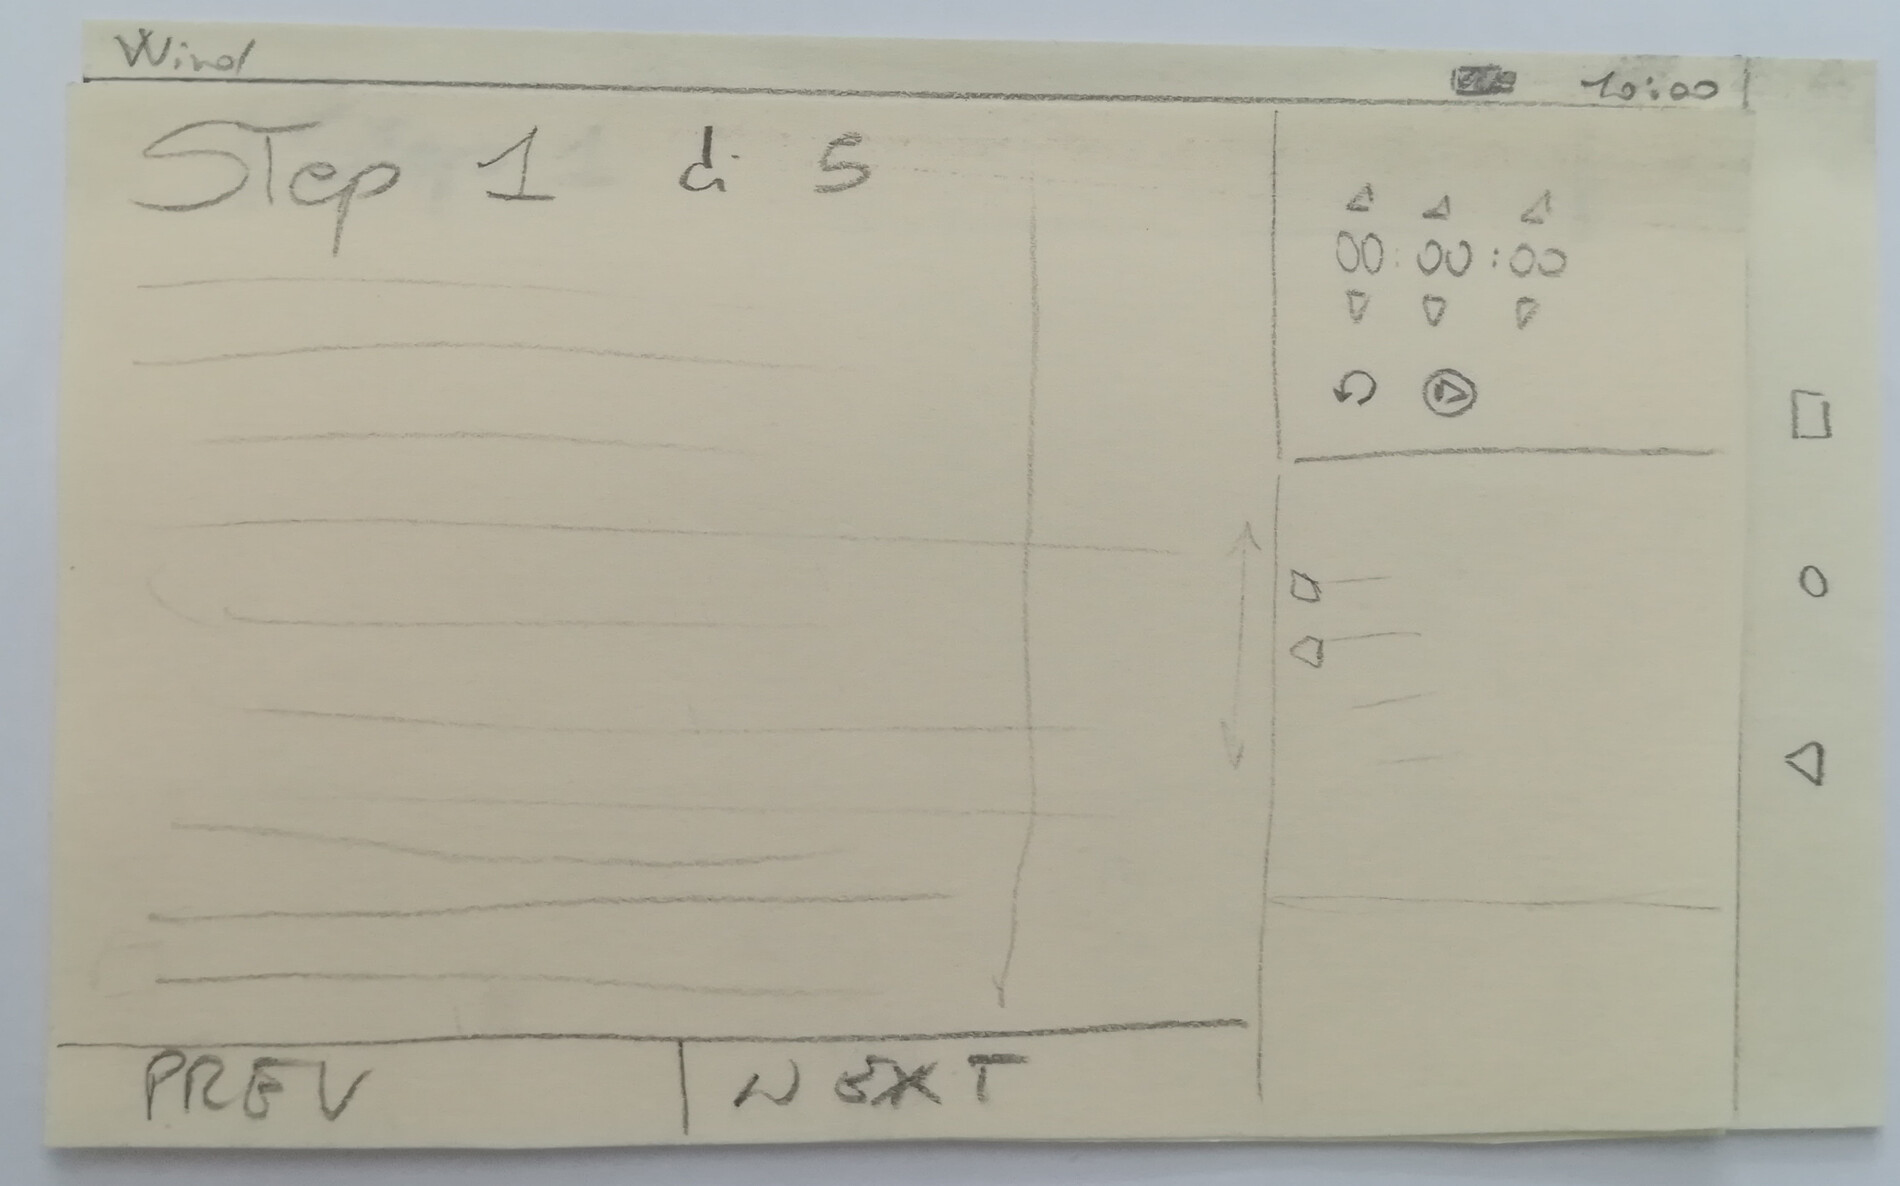
\includegraphics[width=0.78\textwidth]{prototipo1/cuciamo_b}
    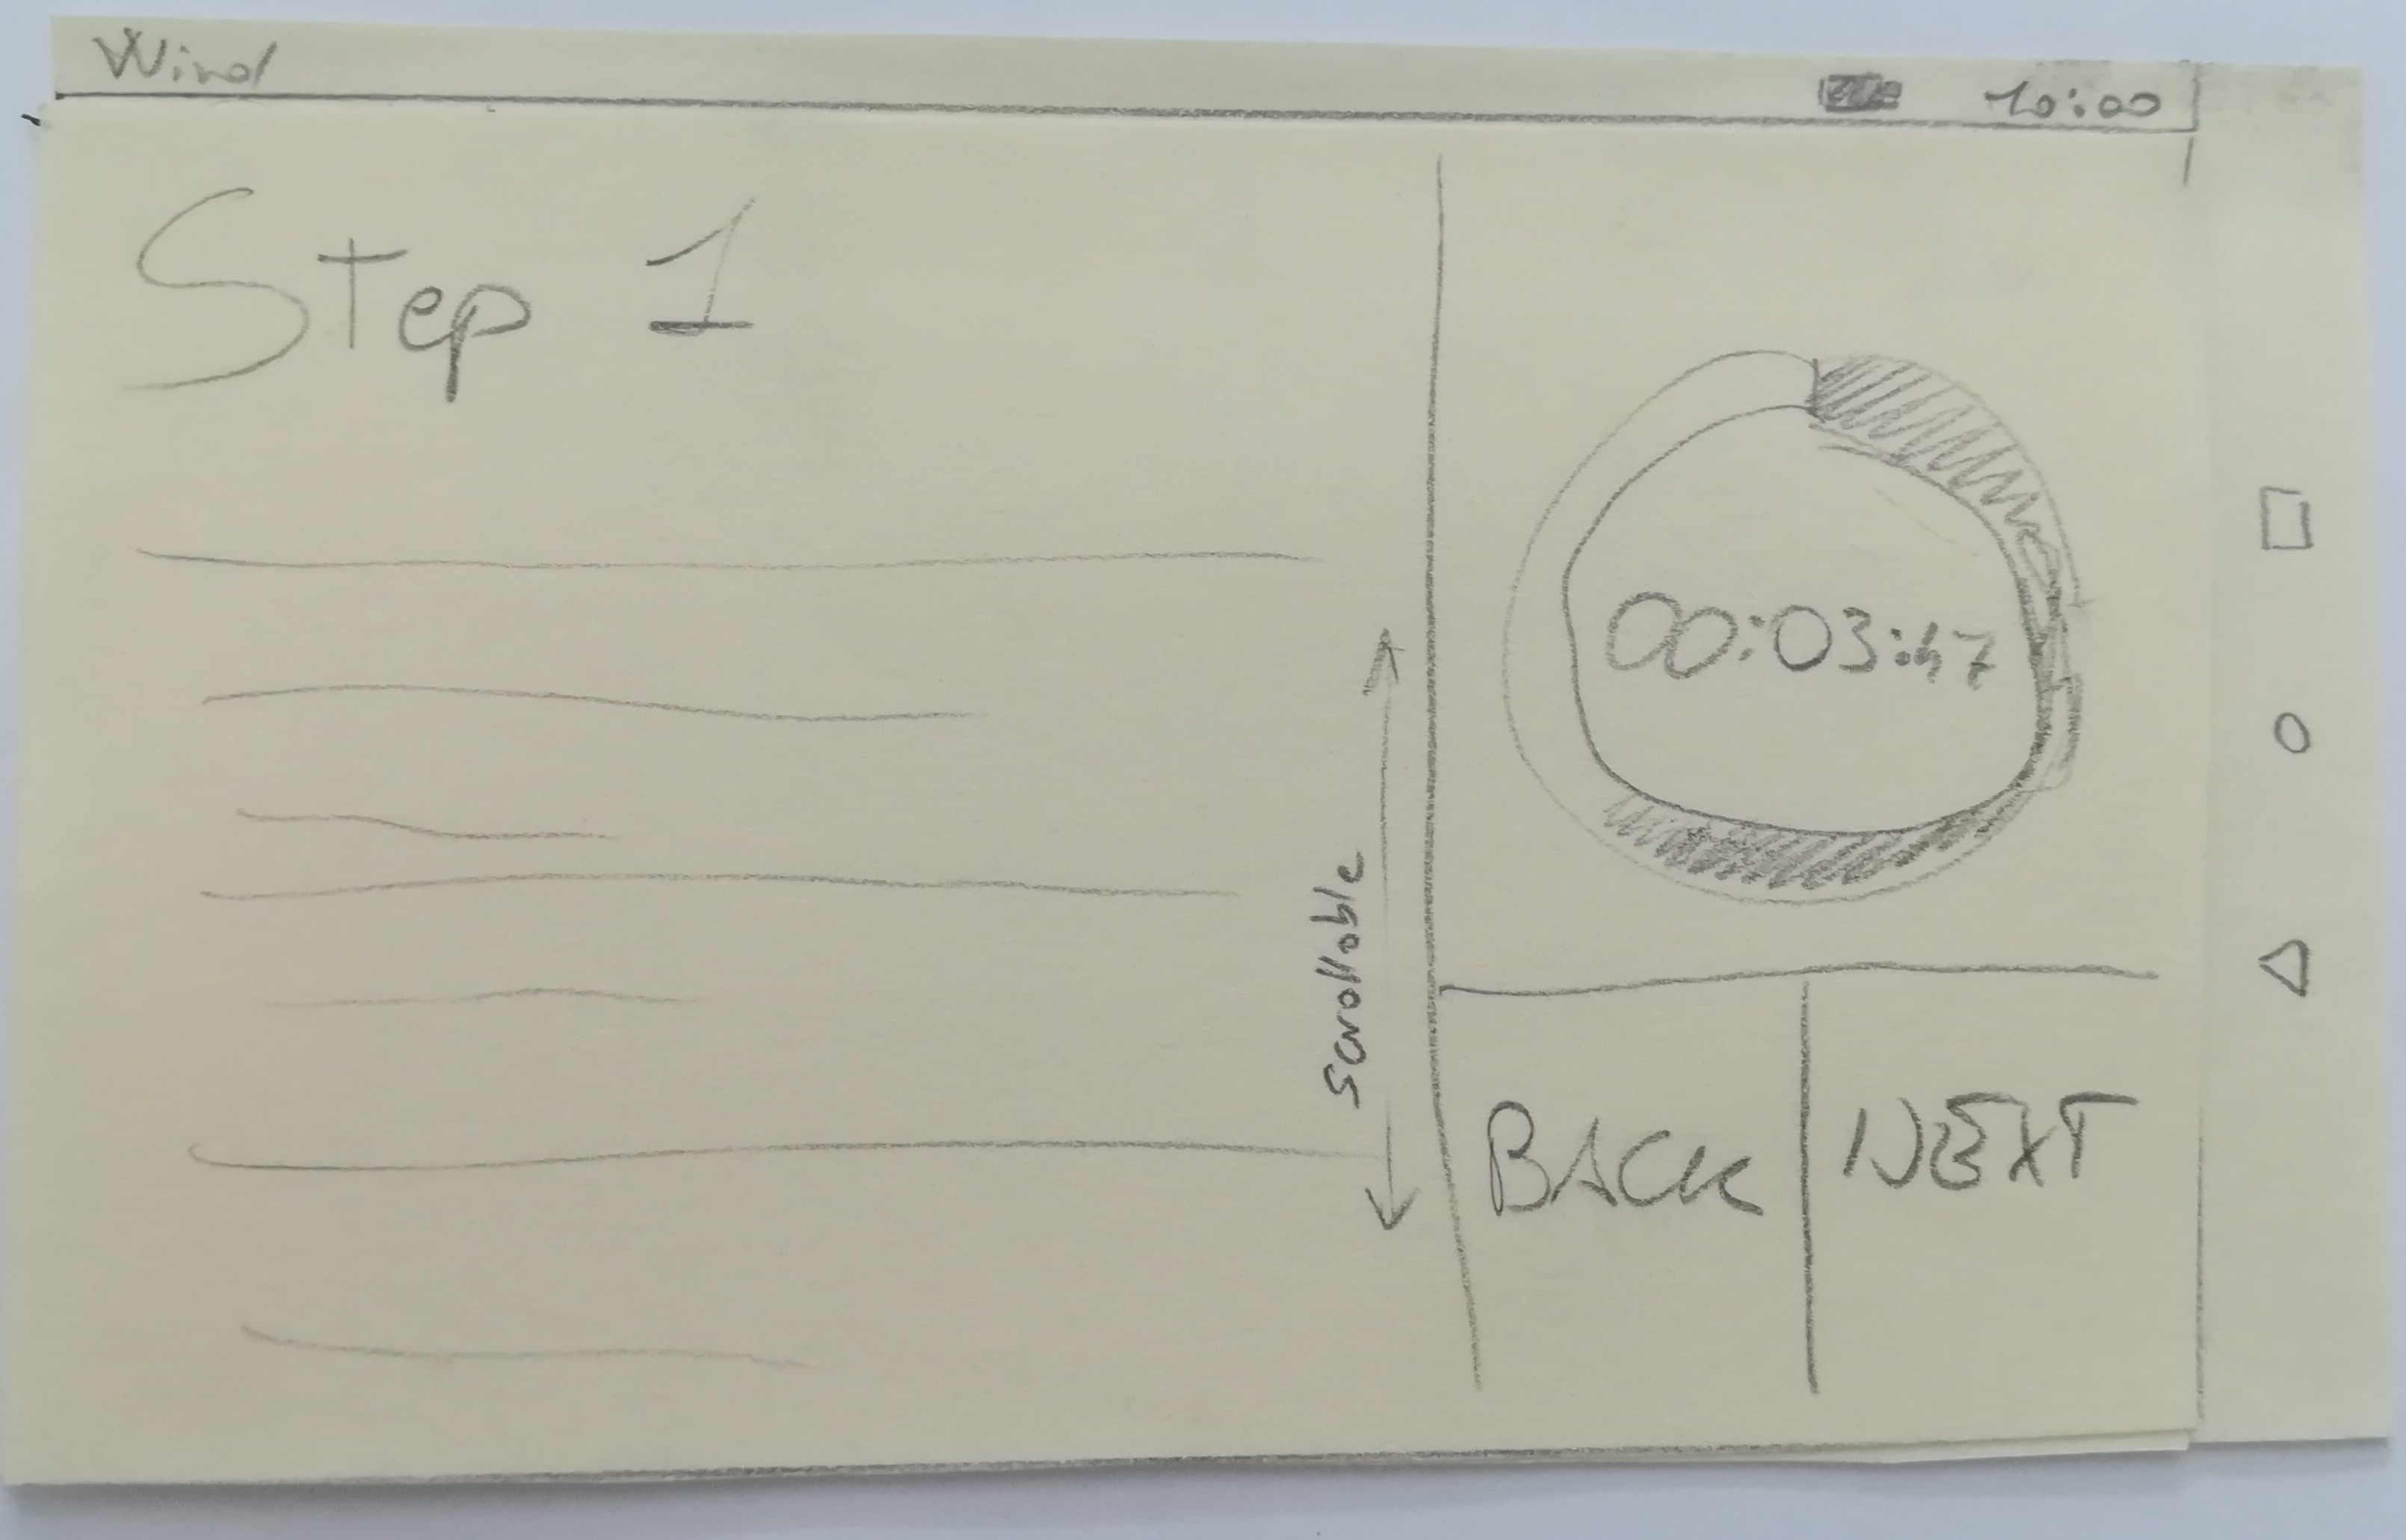
\includegraphics[width=0.78\textwidth]{prototipo1/cuciamo_c}
    \caption{Prime versioni della schermata dell'assistente}
    \label{fig:p1_cuciniamo}
  \end{center}
\end{figure}

\clearpage
In figura \ref{fig:p1_overview} è riportata una visione complessiva del prototipo.

\begin{figure}[ht]
  \begin{center}
    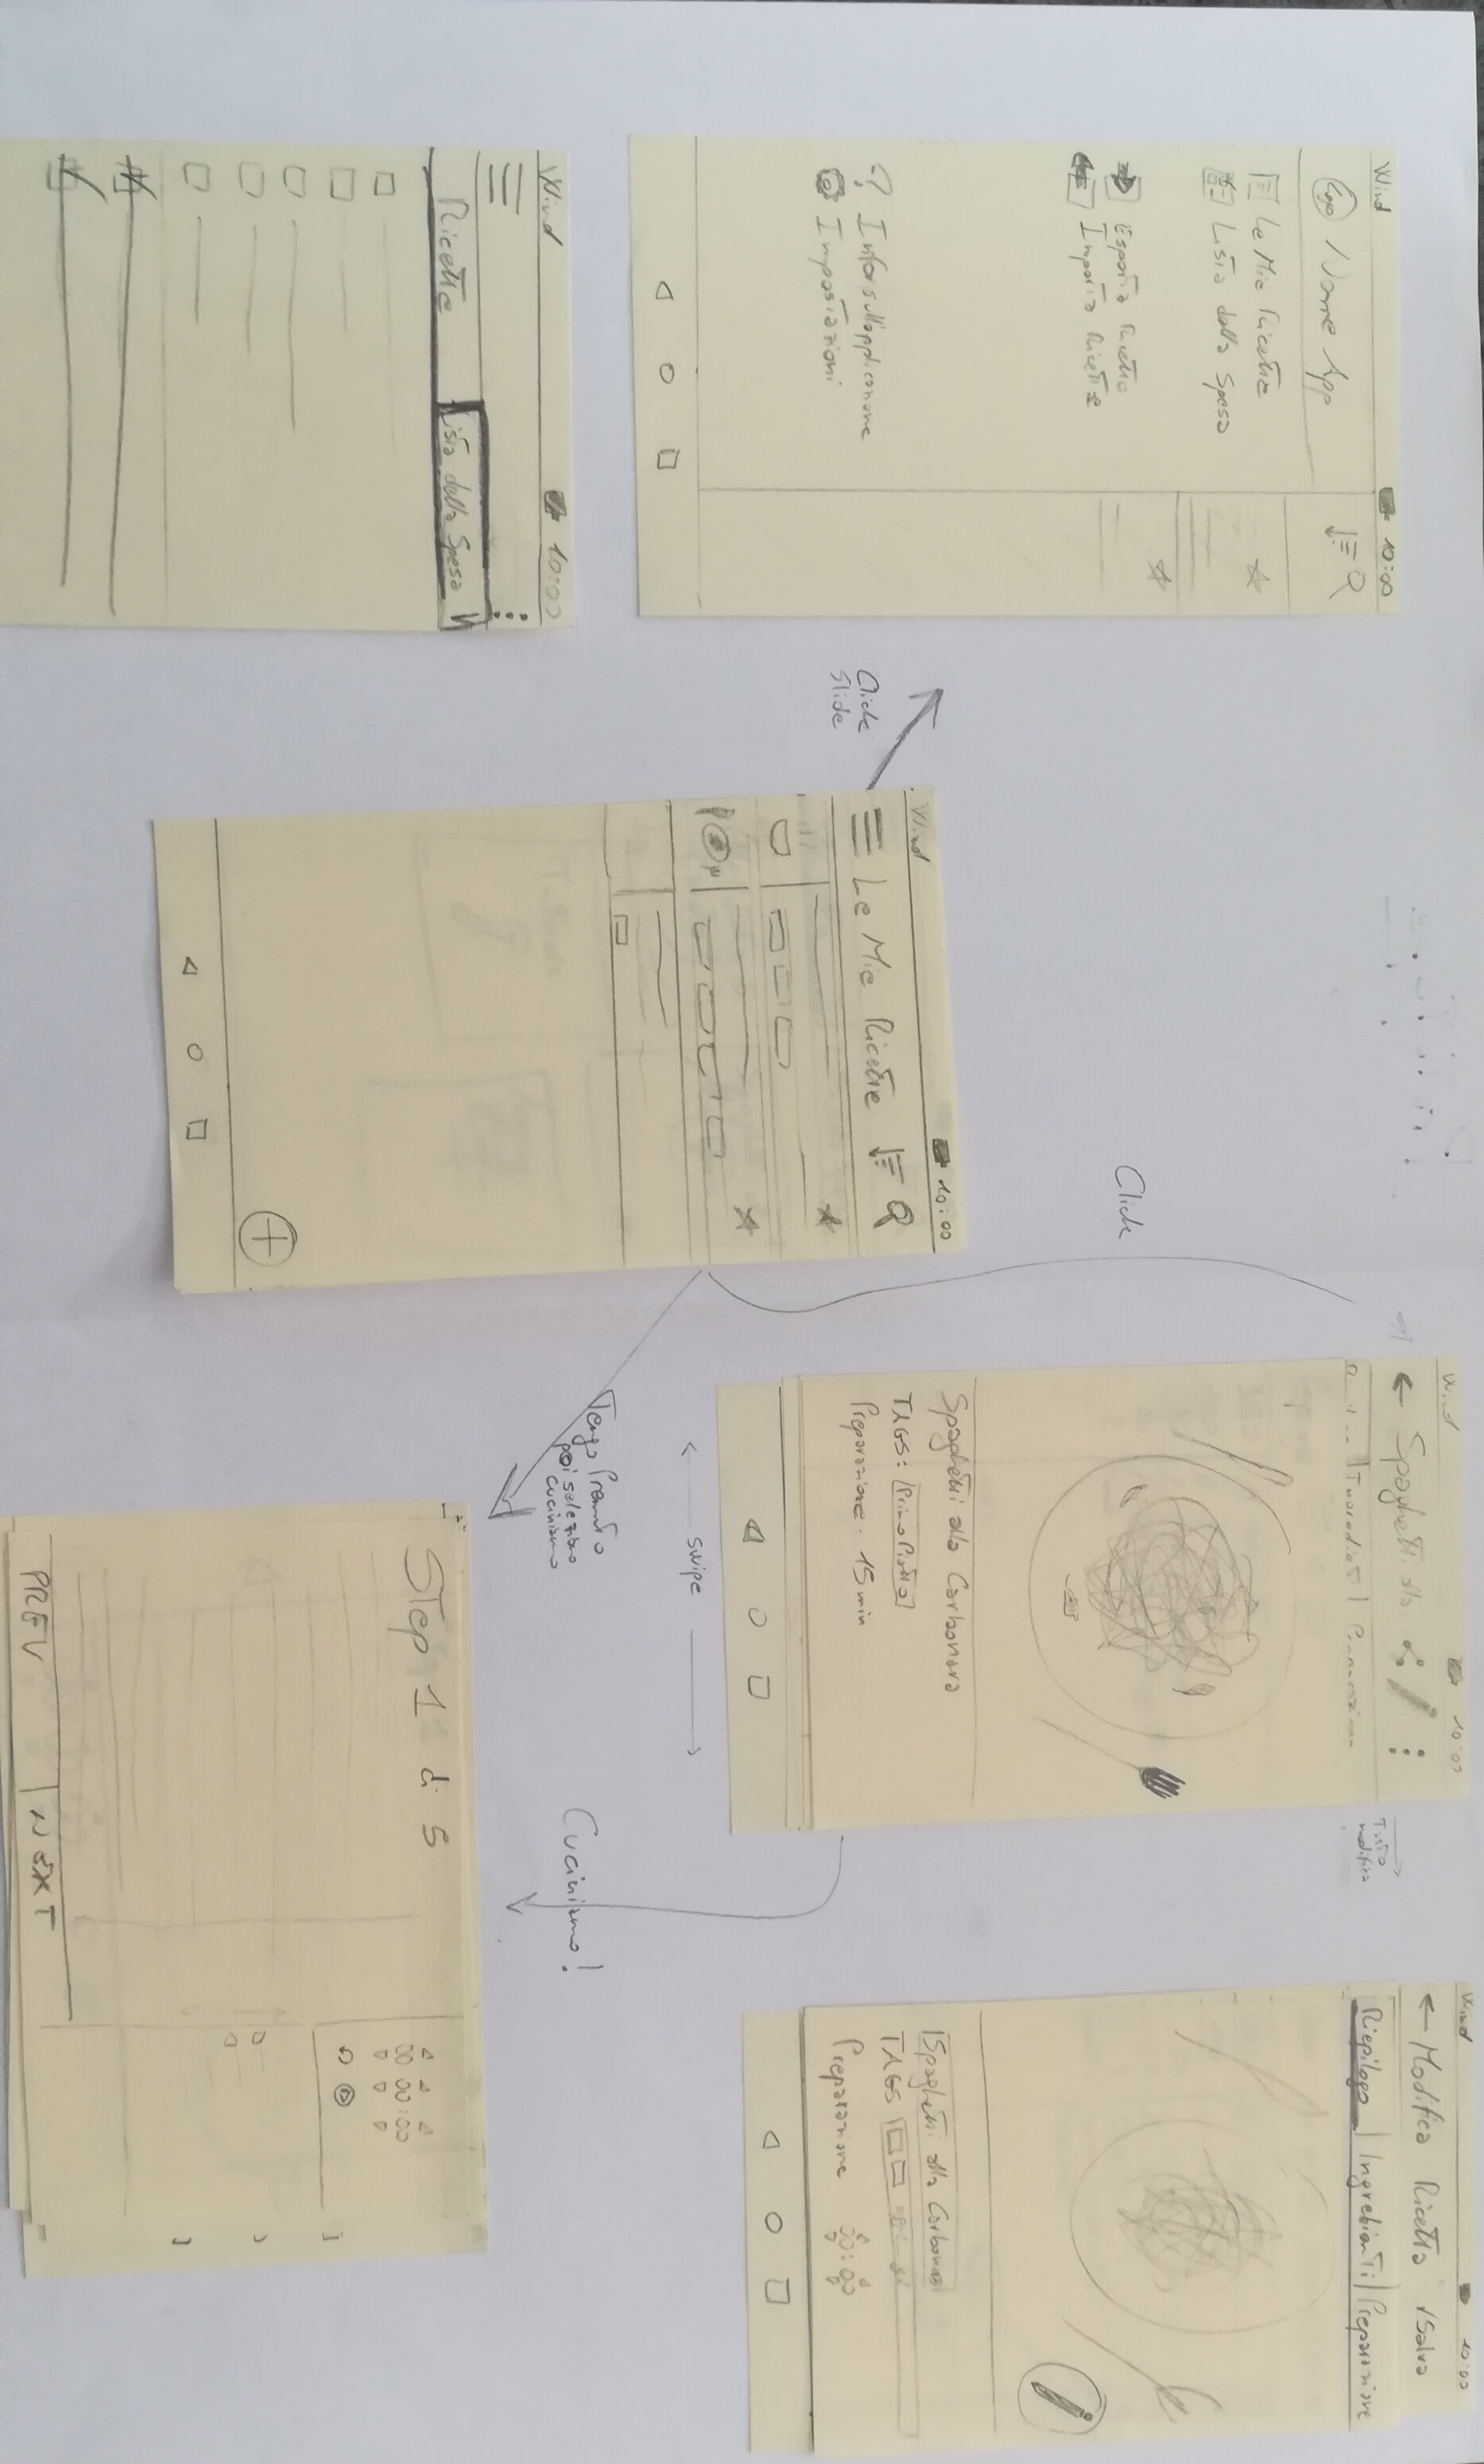
\includegraphics[width=\textwidth]{prototipo1/overview}
    \caption{Rappresentazione globale delle schermate}
    \label{fig:p1_overview}
  \end{center}
\end{figure}

\subsubsection{Valutazione}
Durante i test con gli utenti sono emerse varie considerazioni.
Agli intervistati è stato chiesto di navigare fra le principali schermate, descriverne la funzione e cosa si sarebbero aspettati di trovare.

Segue una lista con le considerazioni più importanti.
\begin{itemize}
  \item Fin da subito è emersa la necessità di rendere più visibile ed accessibile la lista della spesa.
    Infatti per molti utenti è stata l'ultima schermata ad essere aperta.

  \item Le voci "esporta" ed "importa" nel menù laterale non sono sembrate utili a nessun utente.
    La possibilità di esportare od importare più ricette contemporaneamente da eventuali file non si è rivelata d'interesse.

  \item Per gli intervistati la possibilità di cercare ma soprattutto di riordinare ricette non è fondamentale.

\item Nella schermata con l'elenco delle ricette, gli utenti hanno preferito il \textit{floating action button} al tasto in alto a sinistra.
  Molti lo hanno considerato di più facile accesso.

  \item Gli utenti hanno fatto notare che dovrebbe essere possibile aggiungere elementi alla lista della spesa anche se questi elementi non appartengono a nessuna ricetta.

  \item Nella schermata di riepilogo di un ricetta, è stato consigliato di aggiungere anche il tempo di cottura ed eventualmente un grado di difficoltà.

  \item La funzionalità di aumento automatico delle dosi nella schermata degli ingredienti ha subito delle critiche perché certi ingredienti non possono essere moltiplicati esattamente, come le uova e tutti quegli ingredienti dosati in modo discreto (esempio "una mela").
    La principale preoccupazione è che arrotondamenti nei calcoli rovinino le proporzioni delle ricette.
\end{itemize}

Per quanto riguarda la schermata dell'assistente:
\begin{itemize}
  \item sarebbe meglio sapere il numero dello step rispetto al numero totale di step.
    Ad esempio con una barra riempibile oppure con una scritta "Step 1 di 5";

  \item molte persone hanno apprezzato l'idea di sporcare poco lo schermo del cellulare ma hanno anche aggiunto che a prescindere lo utilizzerebbero con le mani il più ulite possibile.

  \item più di qualche intervistato ha espresso la volontà di poter poter saltare da uno step ad un altro senza passare necessariamente per gli step intermedi;

  \item la maggior parte degli utenti preferisce mantenere il cellulare in verticale per poter passare più comodamente ad altre applicazioni, che solitamente vengono utilizzate in modalità \textit{portrait};

  \item meno di metà persone ritiene che il timer nell'applicazione sia utile.
    Infatti molti intervistati hanno dichiarato di usare altre applicazioni per impostare orologi oppure, se stanno cucinando, usano un orologio da parete.
\end{itemize}


\clearpage
\subsection{Secondo Prototipo Low-Fidelity}
\subsubsection{Descrizione del Design}
Il secondo prototipo è stato progettato pensando alle principali considerazioni emerse nella iterazione precedente.
In figura \ref{fig:p2_main_ricette} sono rappresentate due nuove alternative per la schermata principale.

Ora si può accedere alla lista della spesa con molta facilità, basta premere sull'apposita linguetta oppure effettuare un'azione di \textit{swipe} verso destra.
La schermata di destra mostra una disposizione quasi a griglia delle ricette, esteticamente piacevole.
Per ciascuna sono ben visibili il titolo e l'immagine della ricette, però il numero di ricette mostrate contemporaneamente è minore ed inoltre i tag vengono omessi.
In questo design differente l'ultimo elemento della lista funge da tasto di aggiunta di una nuova ricetta.

\begin{figure}[ht]
  \begin{center}
    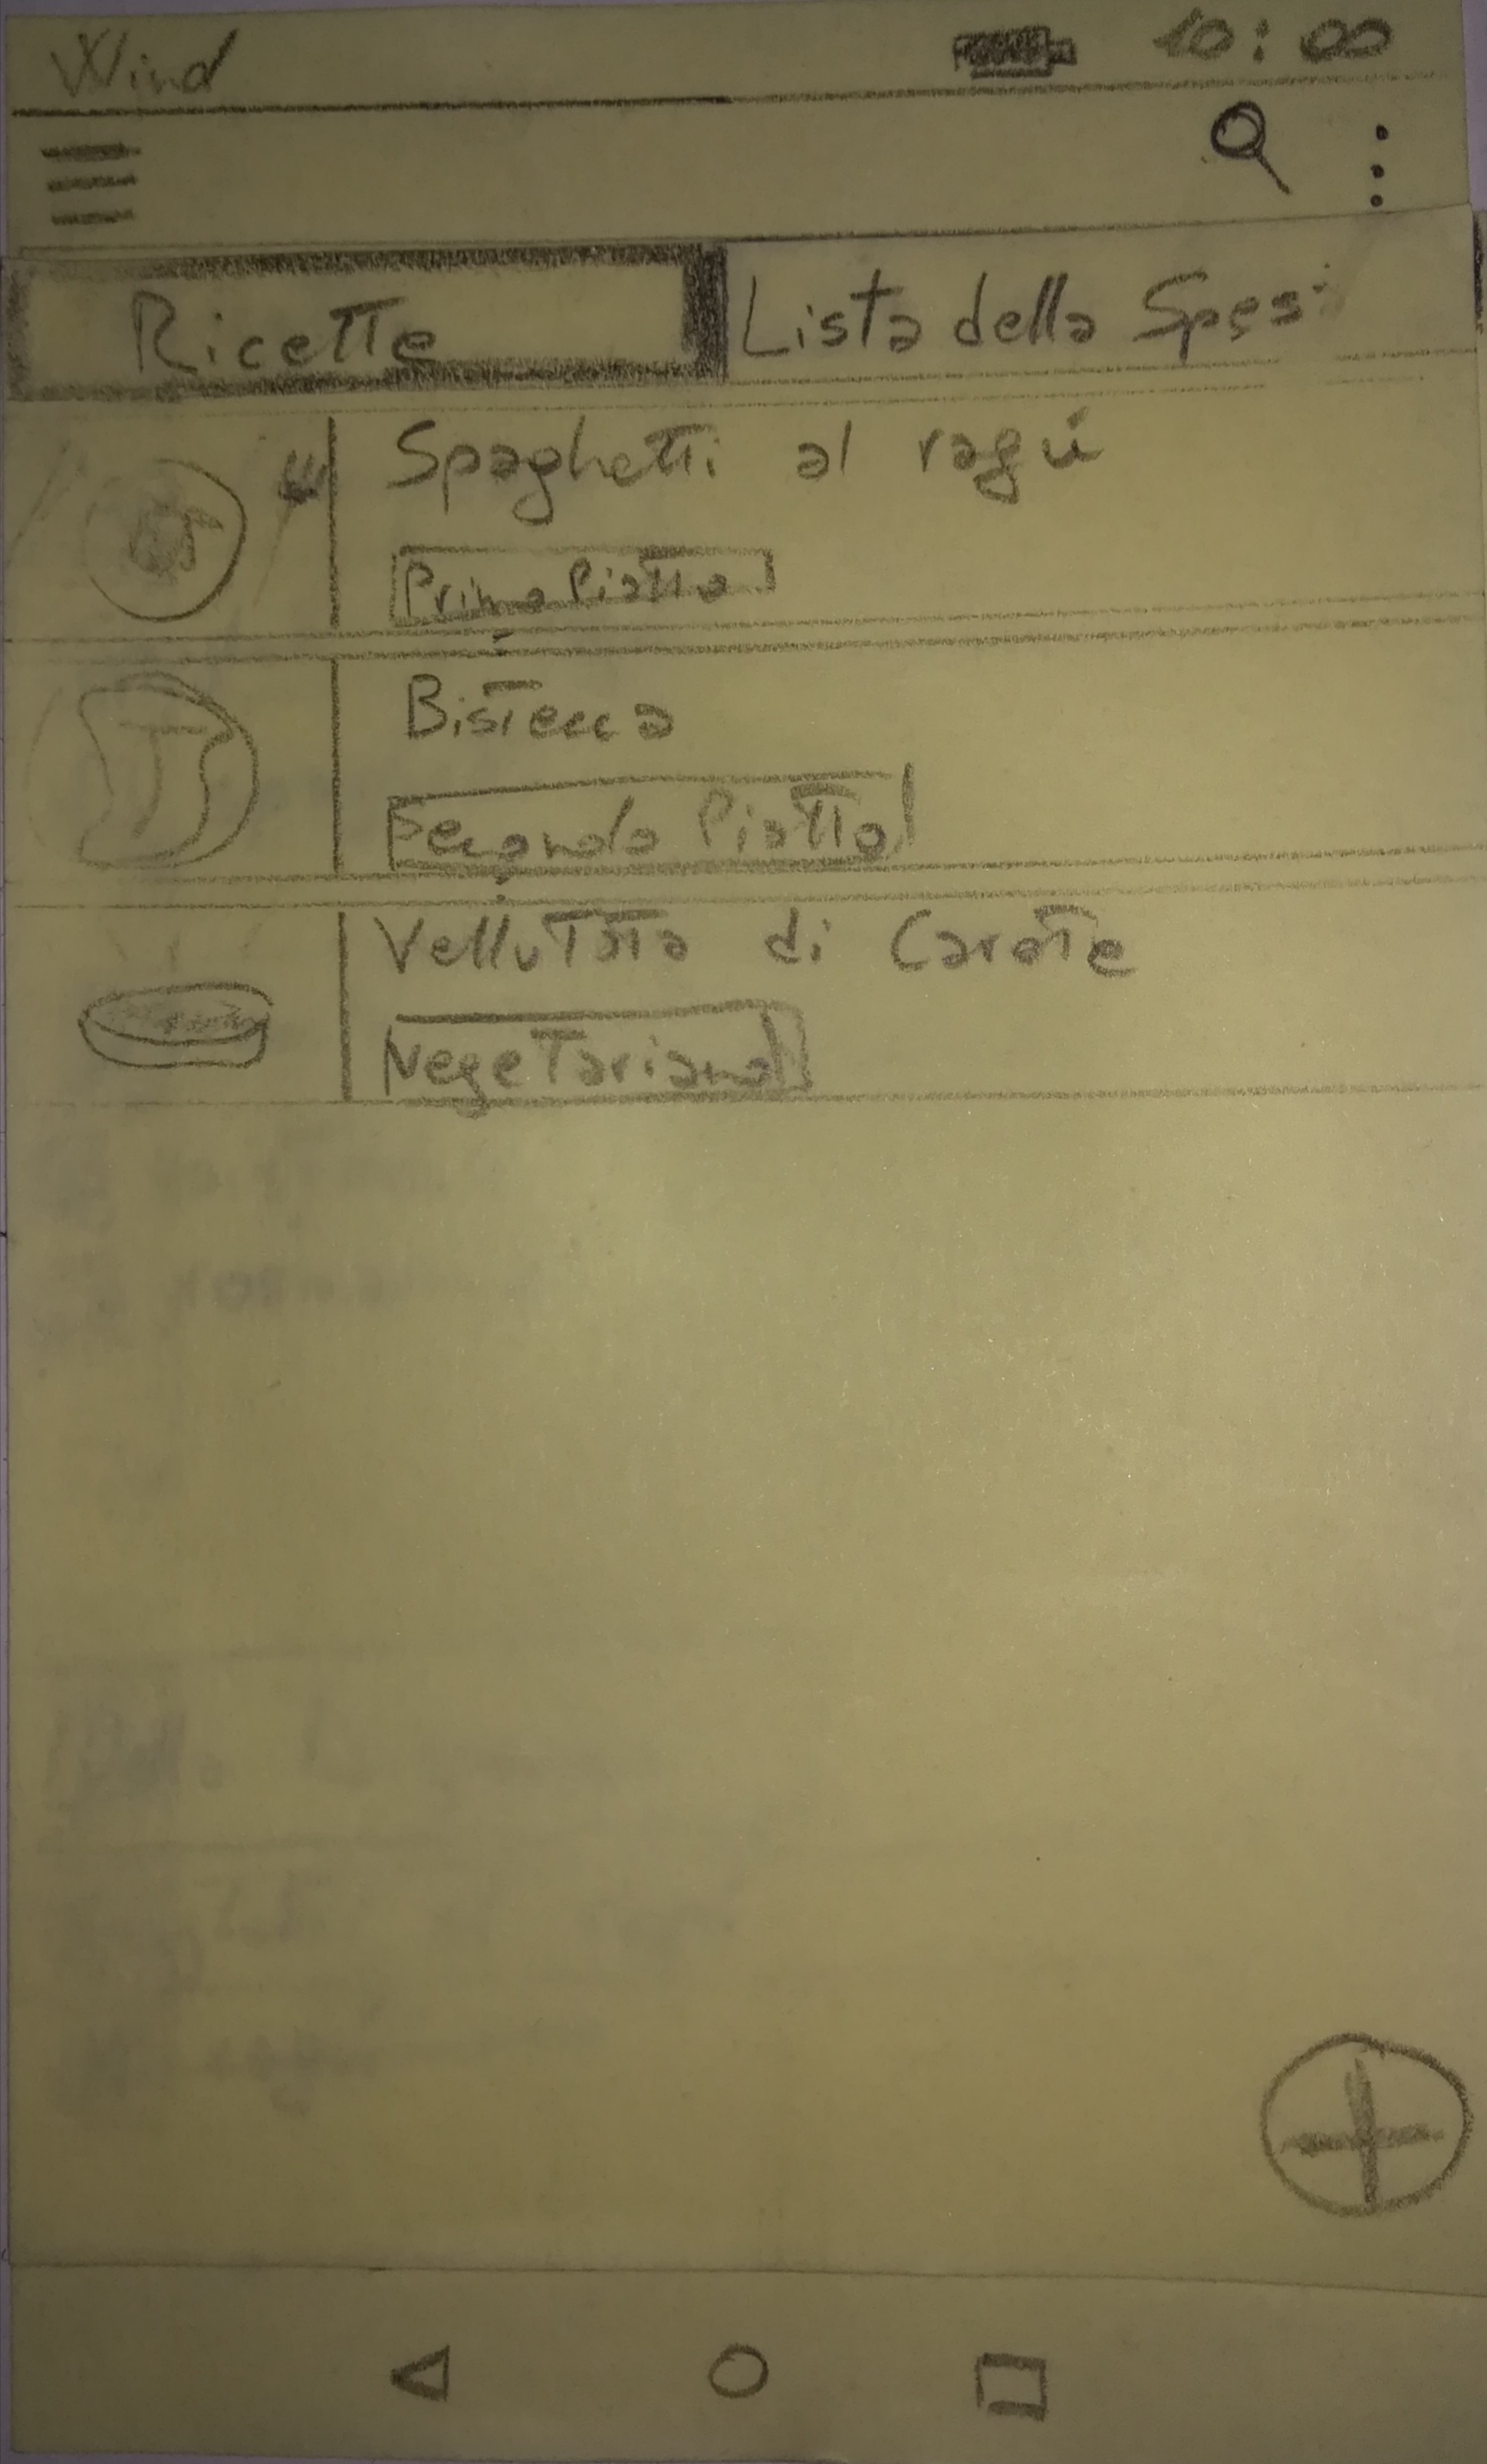
\includegraphics[width=0.49\textwidth]{prototipo2/main_ricette}
    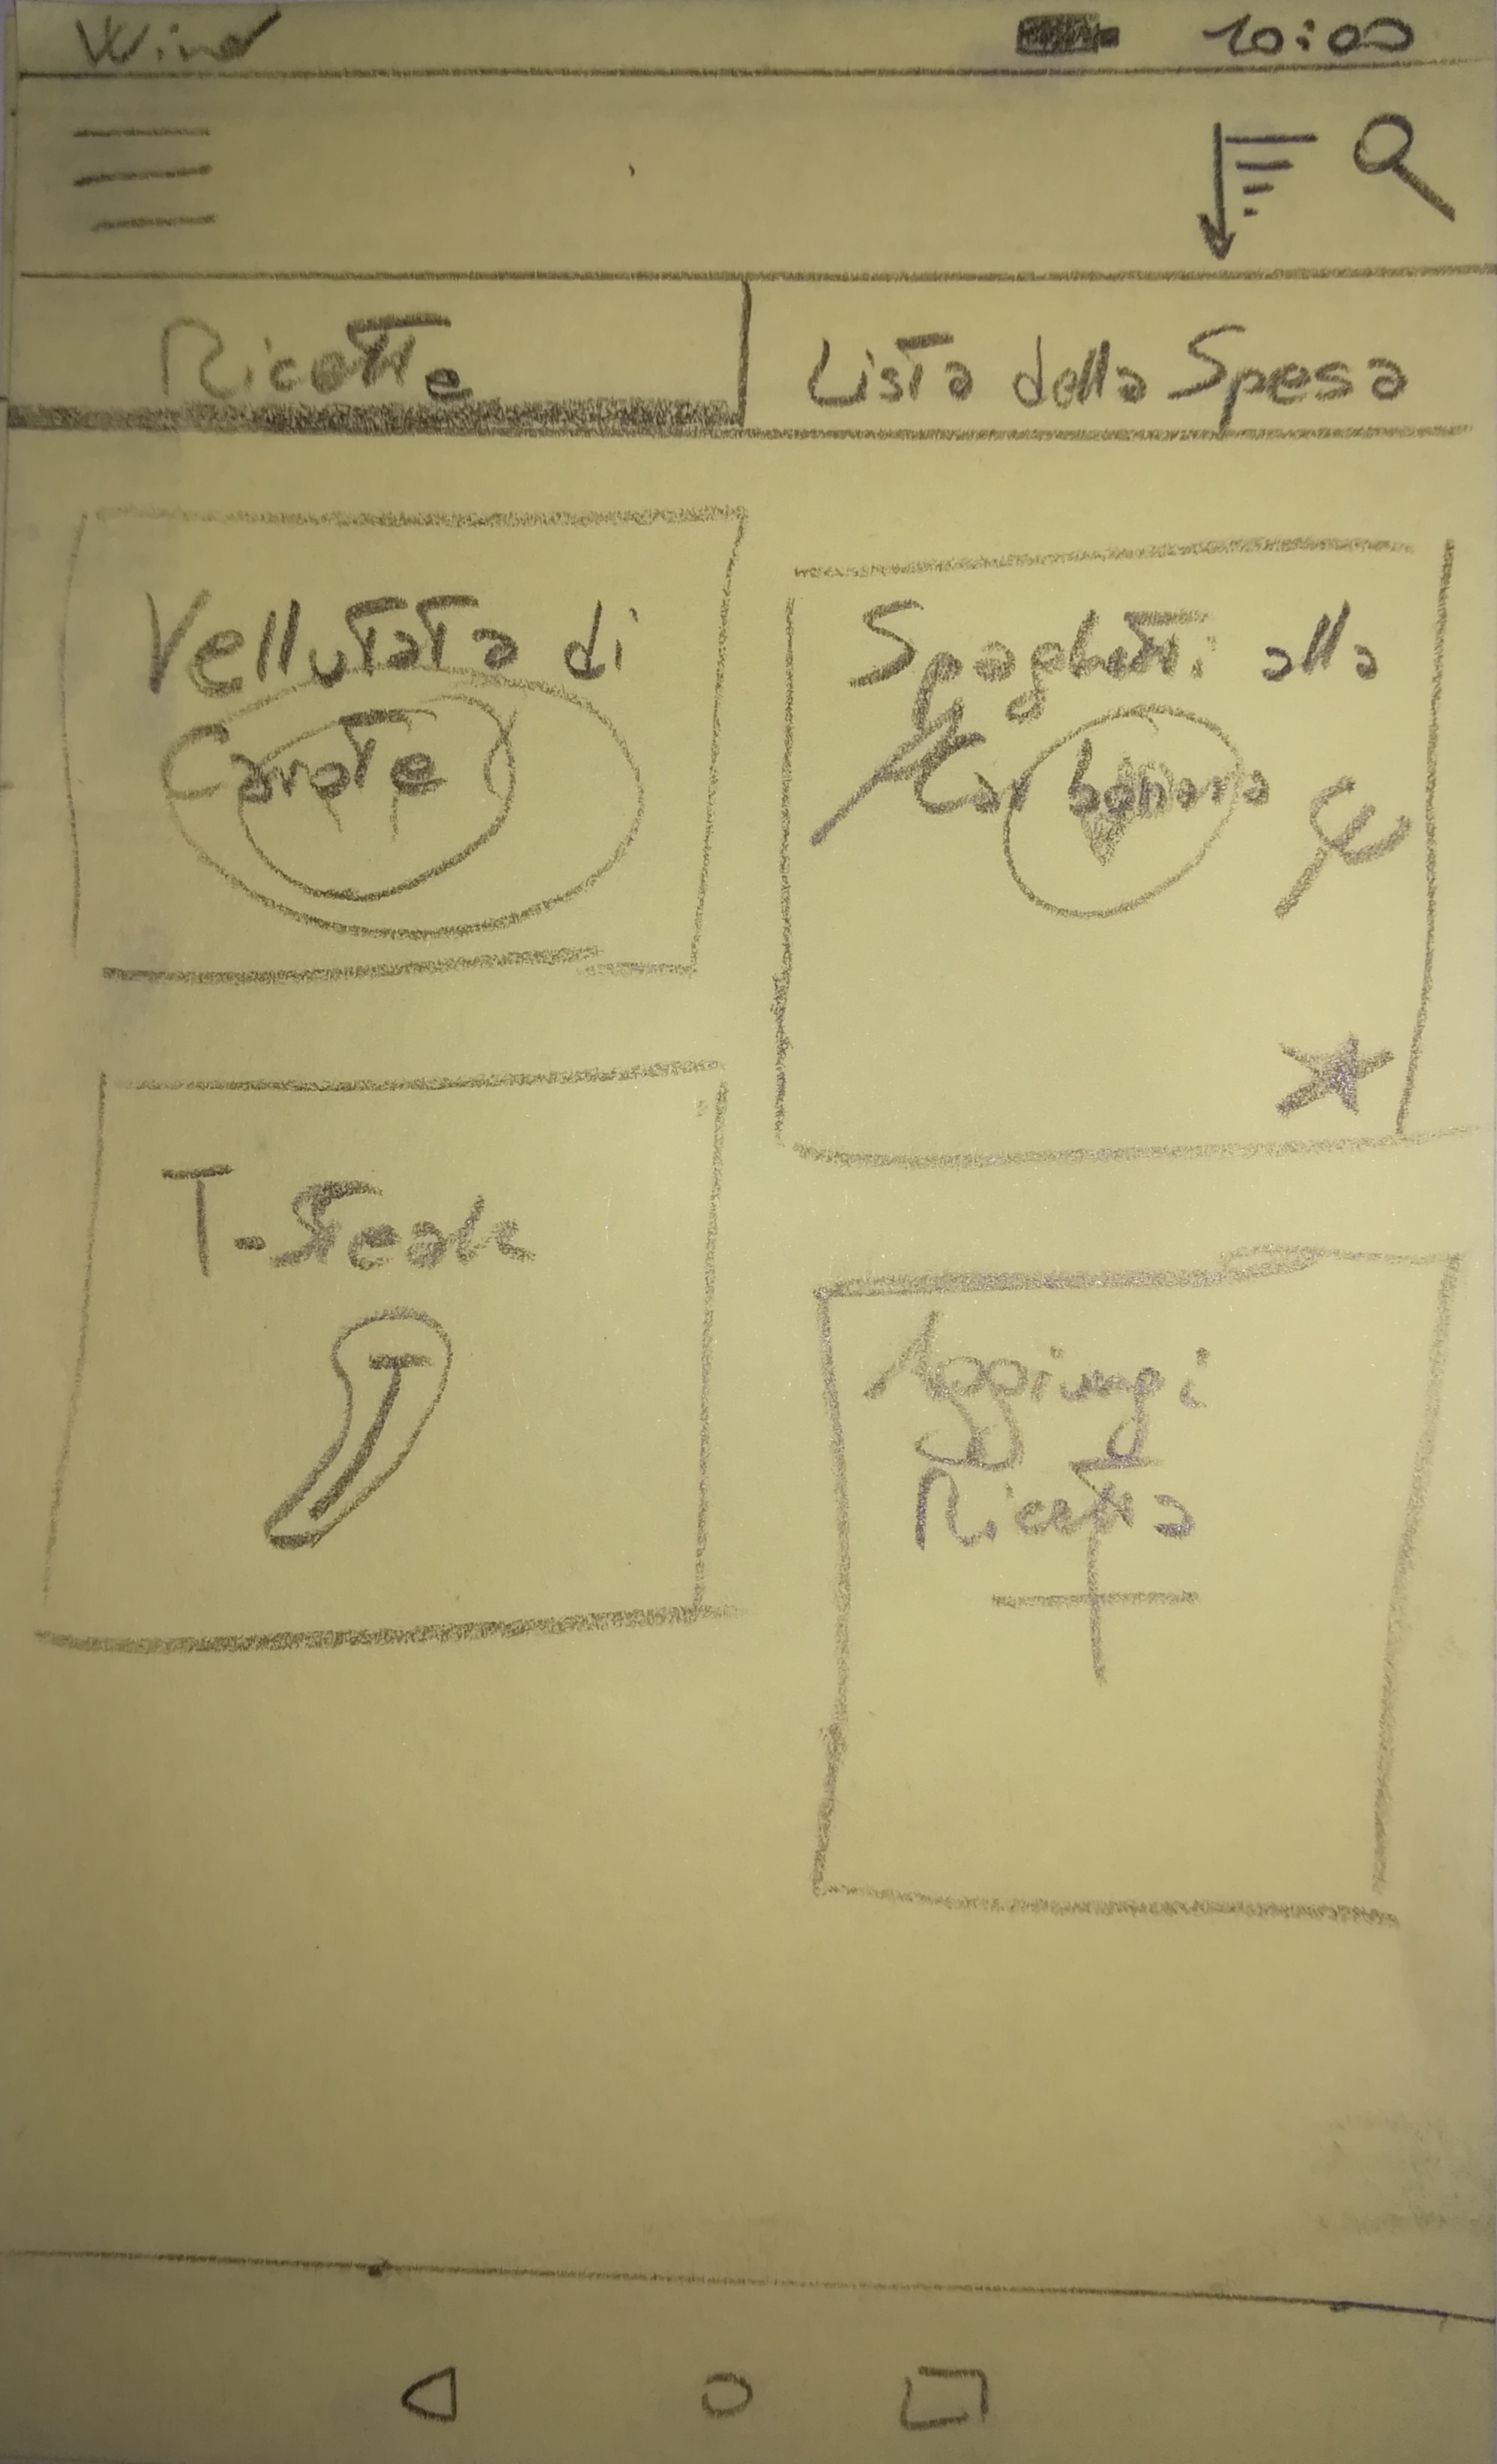
\includegraphics[width=0.49\textwidth]{prototipo2/main_ricette_variant}
    \caption{Nuova schermata principale}
    \label{fig:p2_main_ricette}
  \end{center}
\end{figure}

In figura \ref{fig:p2_main_lista_della_spesa} sono rappresentati il nuovo TODO laterale e la nuova schermata della lista della spesa.
Si può notare che dal TODO laterale sono state rimosse le voci che permettevano di esportare ed importare ricette.

Le due sezioni della lista della spesa sono distinguibili più facilmente grazie a due titoli: "Da Comprare" per il primo gruppo e "In Dispensa" per il secondo.
Notare che ora gli ingredienti sono contenuti nelle rispettive ricette.
Questa scelta è stata fatta considerando la possibilità di dover comprare uno stesso ingrediente per due o più ricette differenti.
Si vuole evitare che l'utente pensi di aver introdotto due volte lo stesso ingrediente erroneamente, altrimenti rischia di non comprare abbastanza ingredienti.
Quando viene aggiunta una spunta ad un ingrediente, questo viene spostato nella sezione "In Dispensa" nella ricetta di appartenenza.

\begin{figure}[ht]
  \begin{center}
    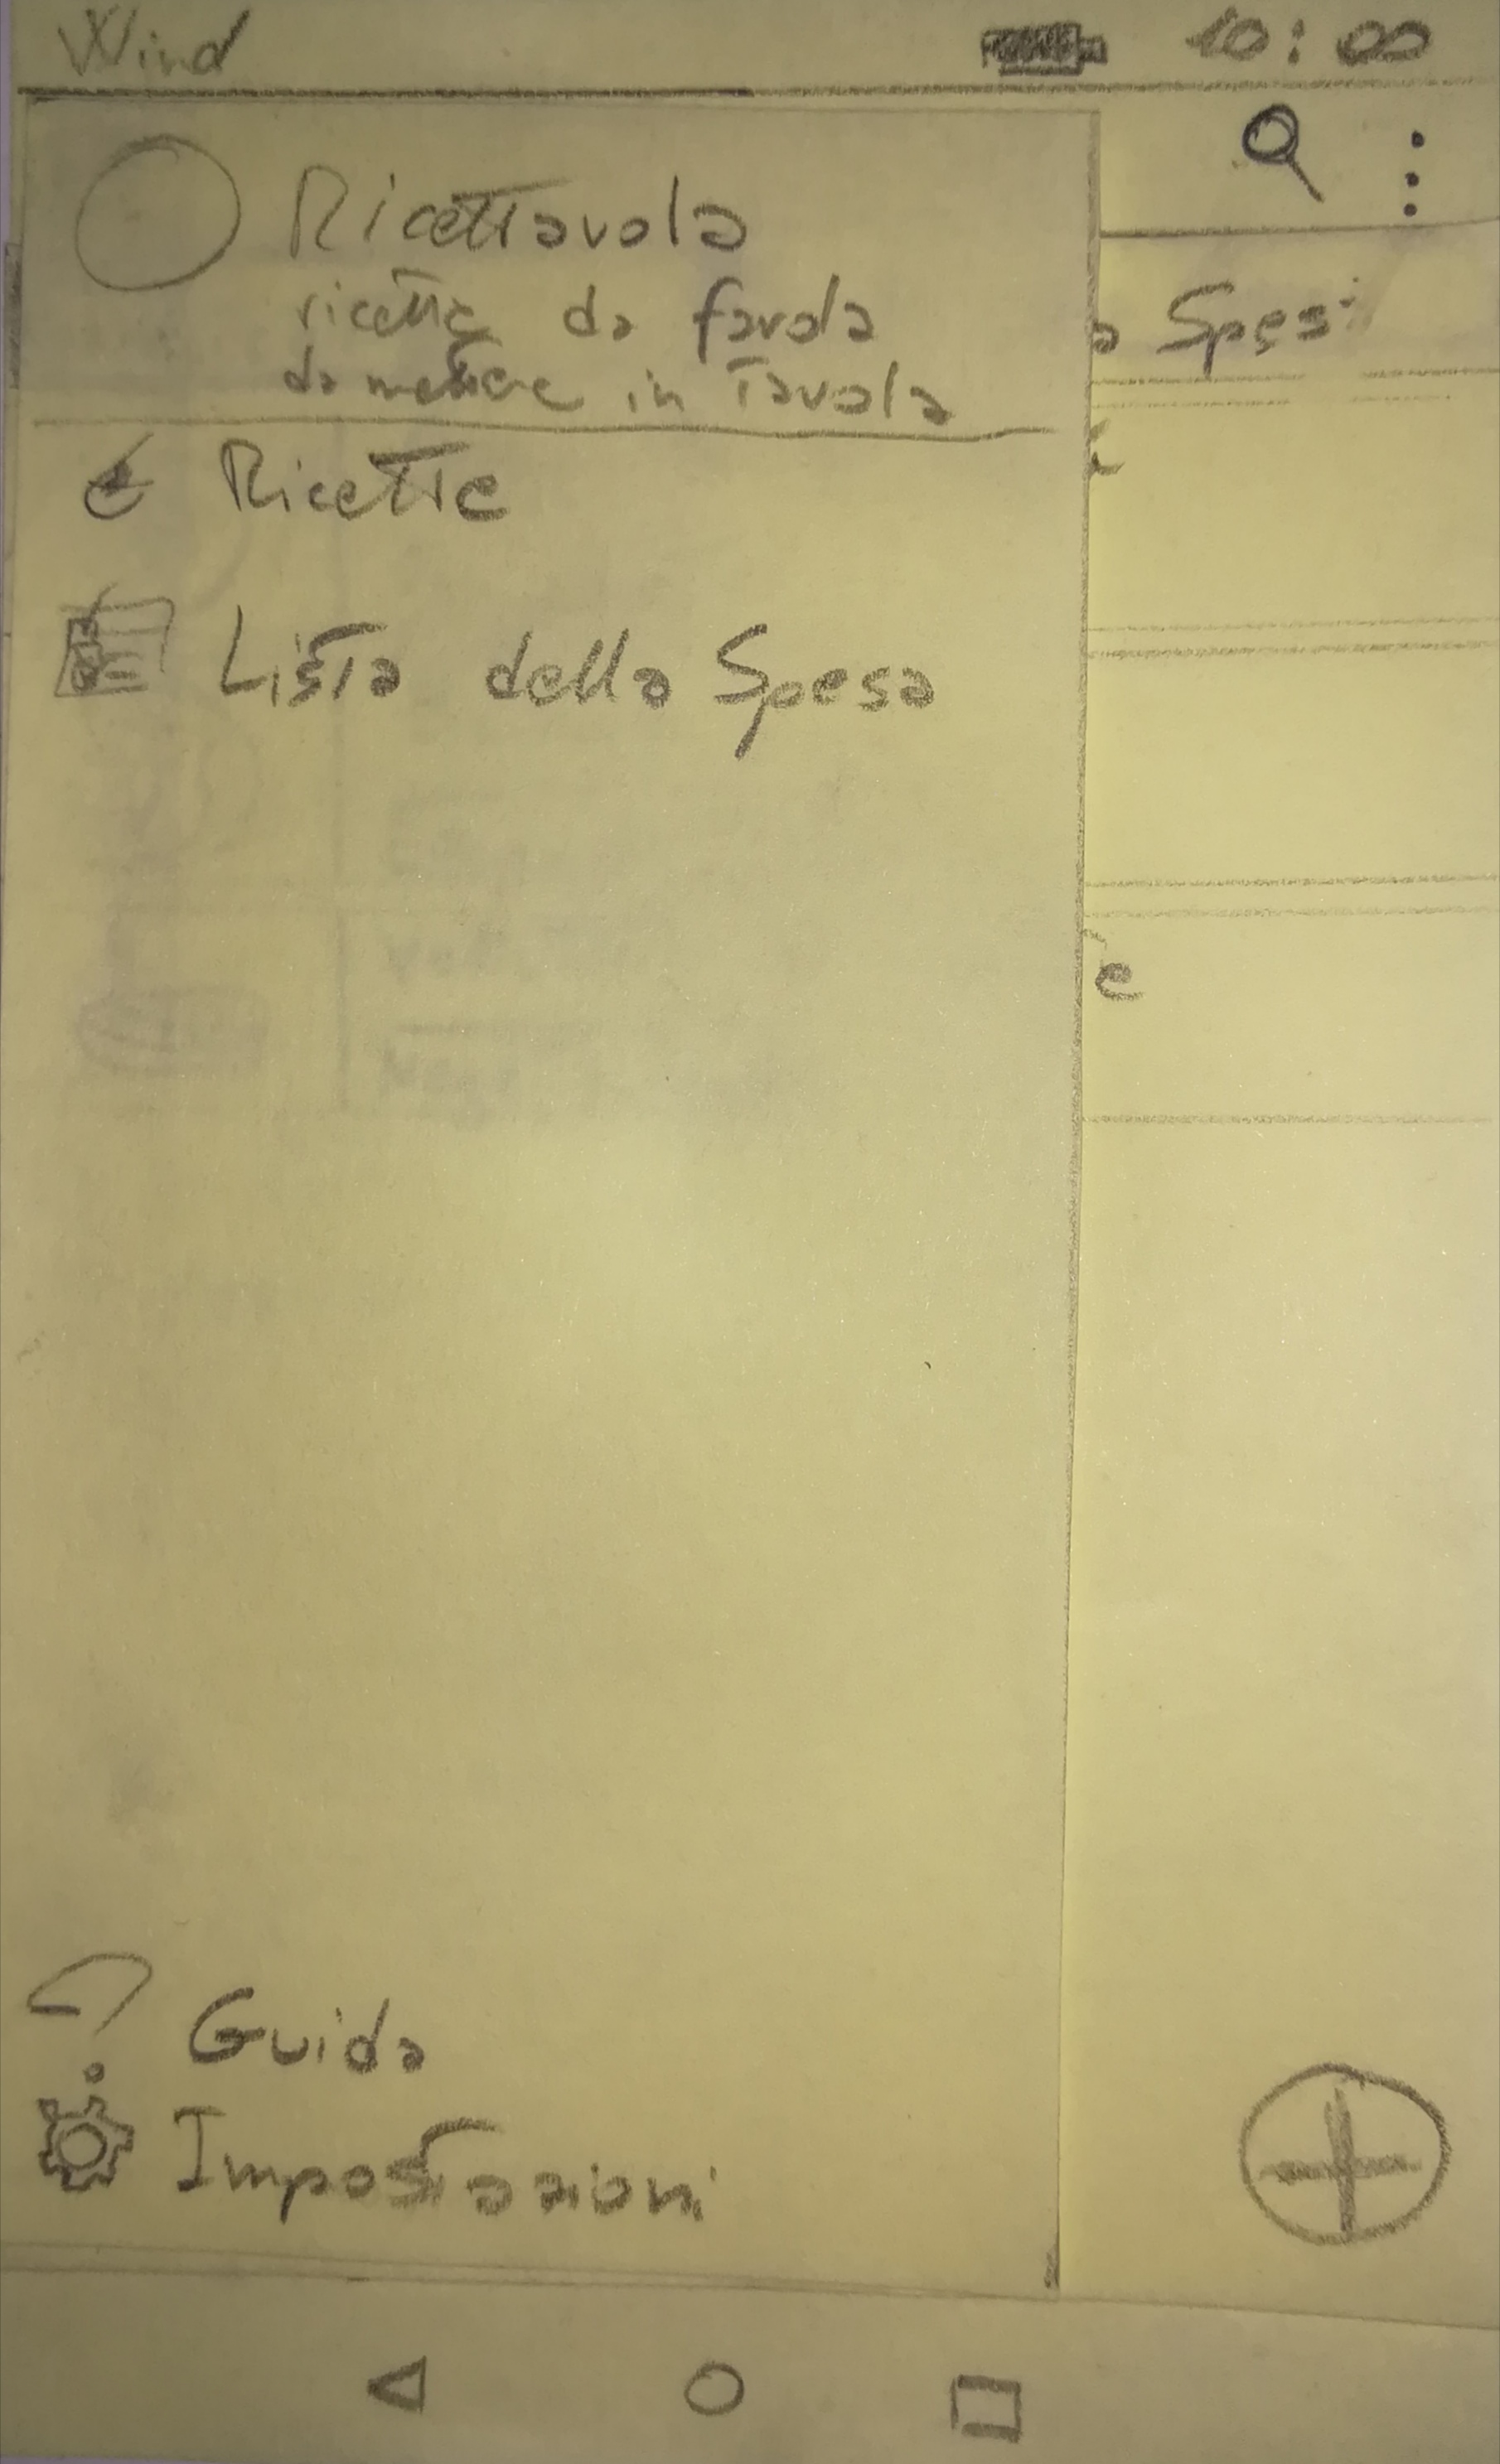
\includegraphics[width=0.49\textwidth]{prototipo2/main_tab}
    \includegraphics[width=0.49\textwidth]{prototipo2/main_lista_della_spesa}
    \caption{Nuovo TODO laterale e schermata della lista della spesa}
    \label{fig:p2_main_lista_della_spesa}
  \end{center}
\end{figure}
\clearpage


Nella figura \ref{fig:p2_ricetta} sono riportate le schermate di visualizzazione di una ricetta.
Nella sezione di riepilogo sono stati aggiunti il tempo di cottura e la difficoltà, mentre in quella degli ingredienti sono stati rimossi i tasti per modificare le quantità degli ingredienti.
Sia nella schermata degli ingredienti che in quella della preparazione è presente una nuova zona in cui possono essere aggiunte delle note provvisorie.
Nelle note possono essere aggiunte piccole modifiche alla ricetta di cui non si è ancora sicuri oppure possibili sperimentazioni future.

\begin{figure}[ht]
  \begin{center}
    \includegraphics[width=0.325\textwidth]{prototipo2/ricetta_riepilogo}
    \includegraphics[width=0.325\textwidth]{prototipo2/ricetta_ingredienti}
    \includegraphics[width=0.325\textwidth]{prototipo2/ricetta_preparazione}
    \caption{Da sinistra a destra: riepilogo, ingredienti, preparazione}
    \label{fig:p2_ricetta}
  \end{center}
\end{figure}

Infine viene illustrata la nuova versione delle schermate della assistente, riportata in figura \ref{fig:p2_cuciniamo}.
Dopo aver premuto il tasto "Cuciniamo" nella schermata di preparazione della ricetta si aprirà una schermata simile a quella a sinistra in figura \ref{fig:p2_cuciniamo} ma indicante il primo step della ricetta.
Effettuando un'azione di scorrimento a destra si ottiene esattamente la schermata raffigurata.
In testa alla schermata è stata aggiunta una barra in cui ogni pallino rappresenta uno step.
Nel caso in cui la ricetta avesse molti step si potrebbe far scorrere la barra a destra e a sinistra per visionarli tutti.
I pallini vengono riempiti se corrispondono a step precedenti oppure a quello attuale.
Nella parte bassa dello schermo sono riportati tutti gli ingredienti della ricetta.
L'utente potrà rimuoverli mano a mano che vengono utilizzati.
Si fa notare che la transizione da uno step all'altro, per venire incontro alle esigenze emerse nell'iterazione precedente, può avvenire in due modi: tramite \textit{swipe} oppure tramite tocco di uno dei pallini della barra superiore.

La seconda immagine in figura \ref{fig:p2_cuciniamo} riporta la possibilità di far comparire un TODO laterale in cui segnare eventuali note.
Queste, a seconda della sezione in cui vengono scritte, sono aggiunte nelle schermate "Ingredienti" oppure "Preparazione" di figura \ref{fig:p2_ricetta}.

\begin{figure}[ht]
  \begin{center}
    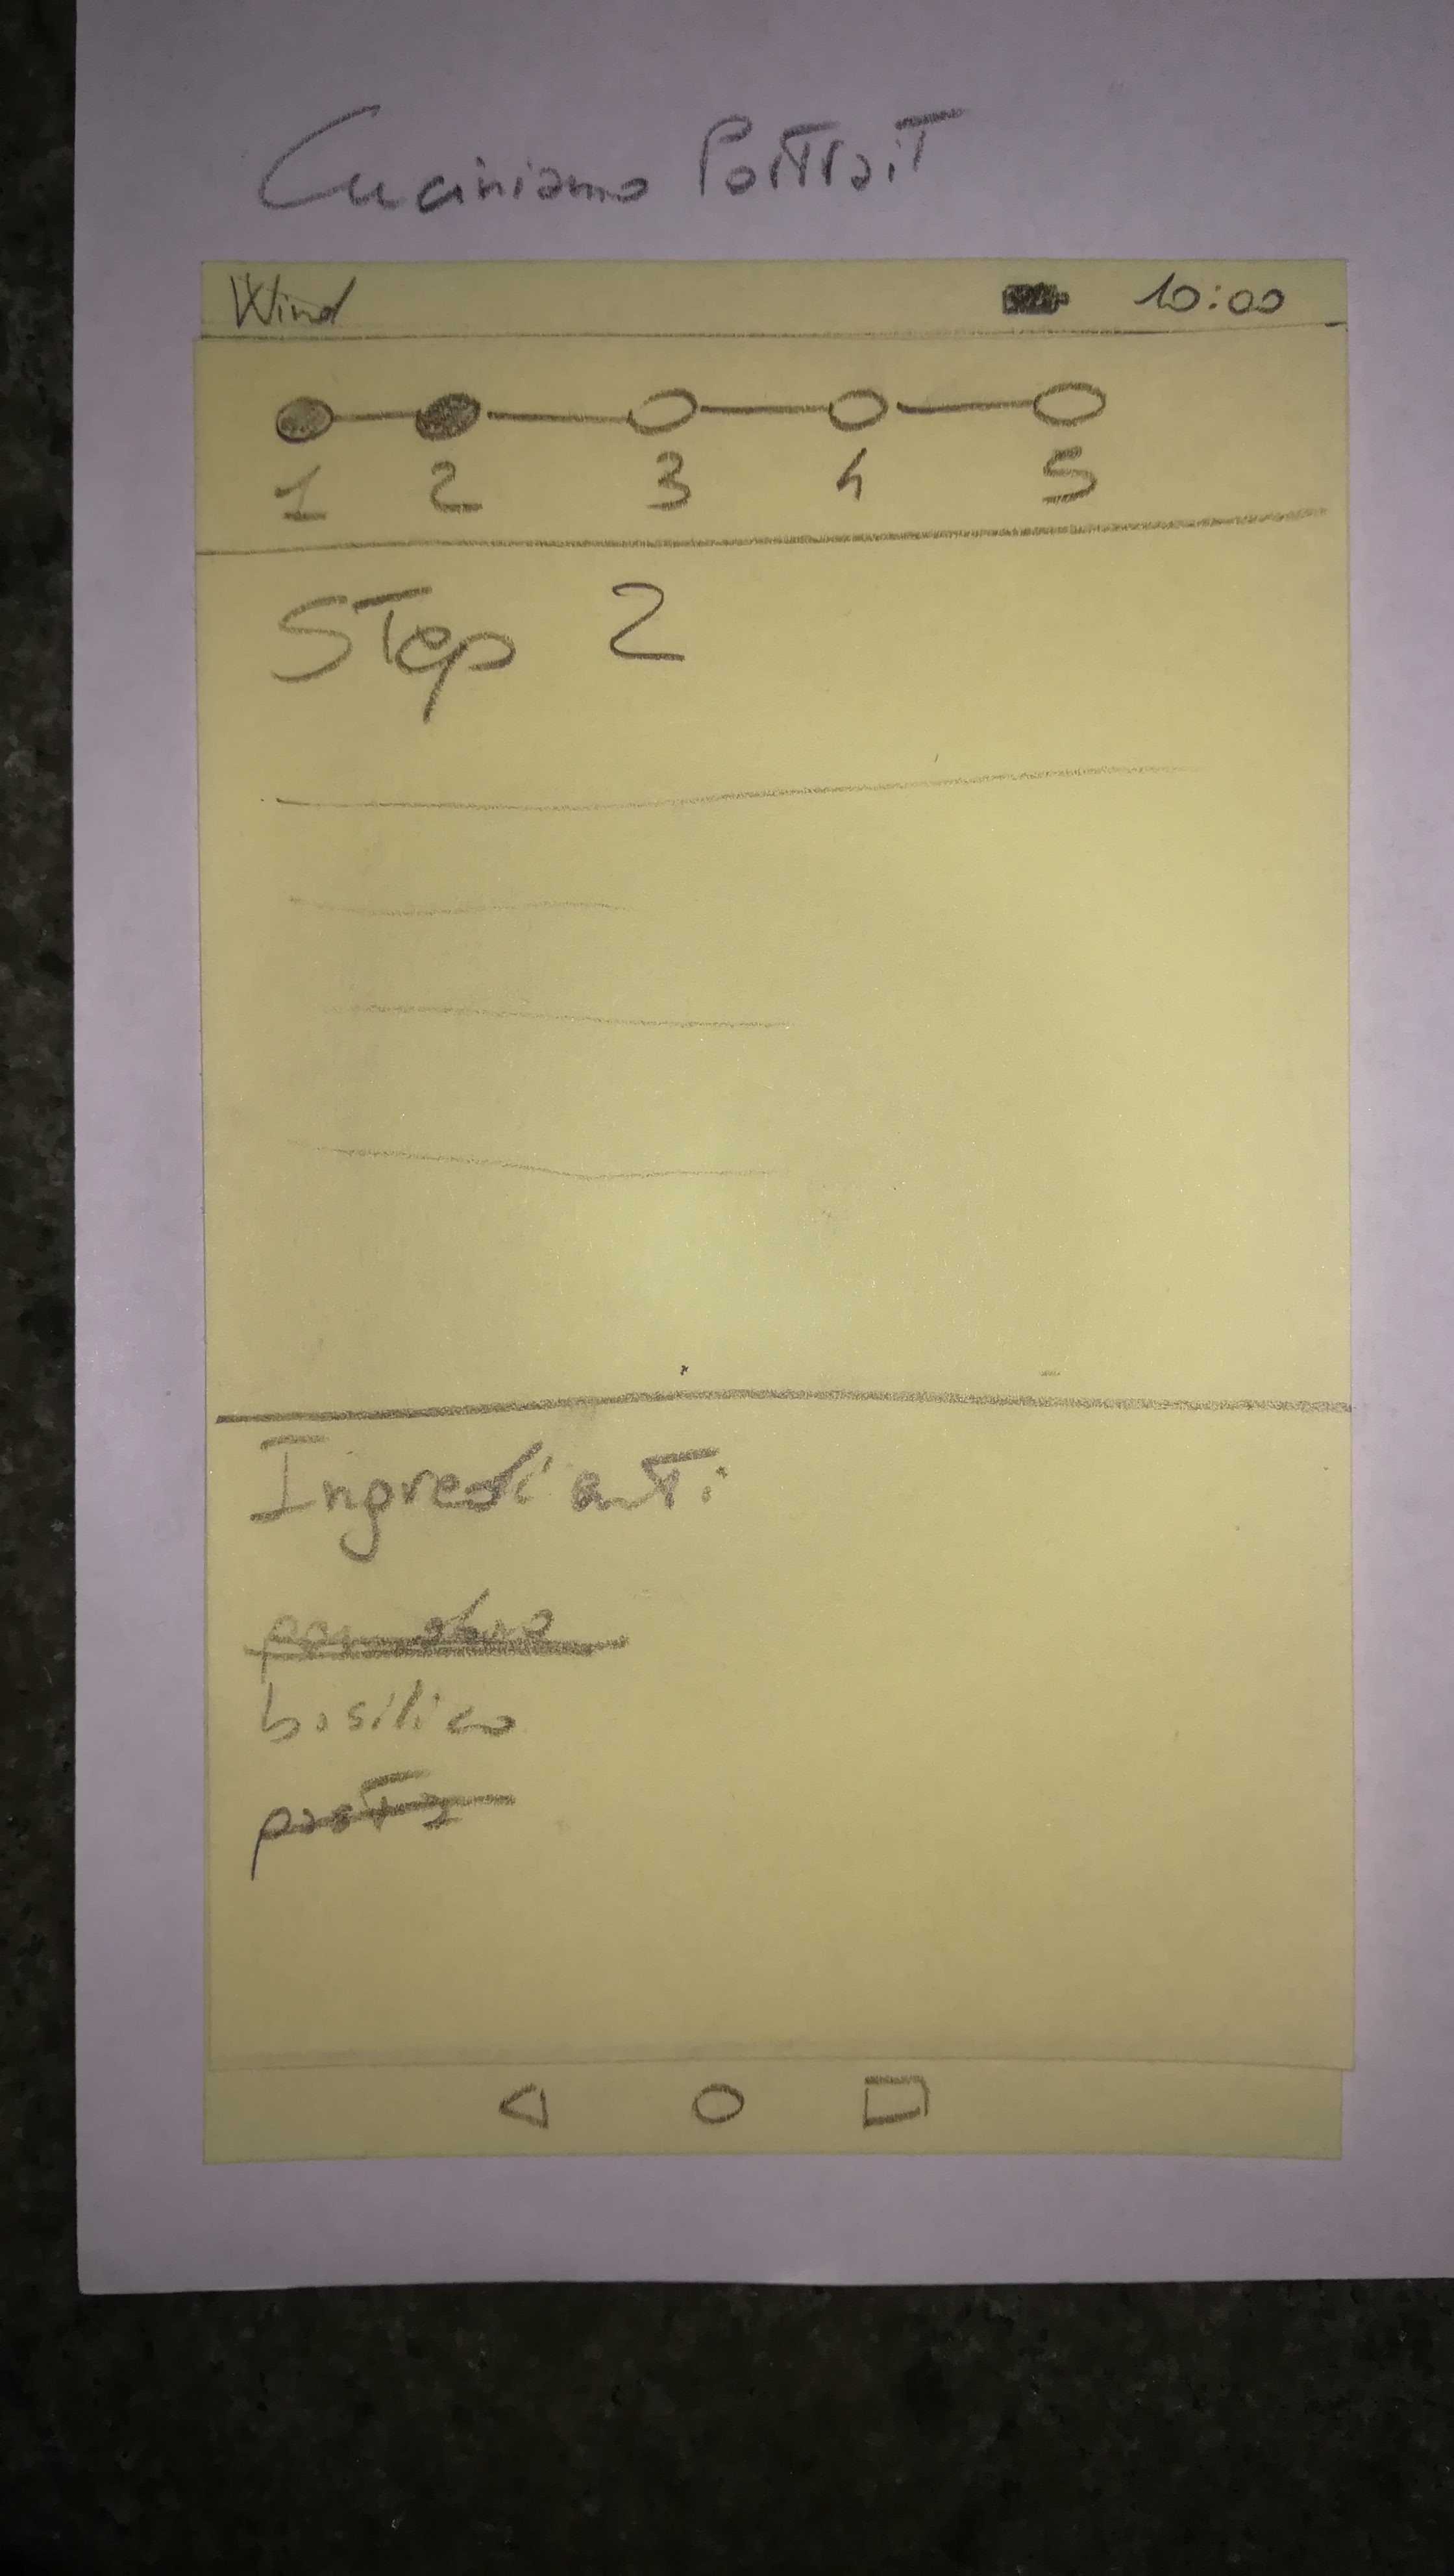
\includegraphics[width=0.4\textwidth]{prototipo2/cuciniamo}
    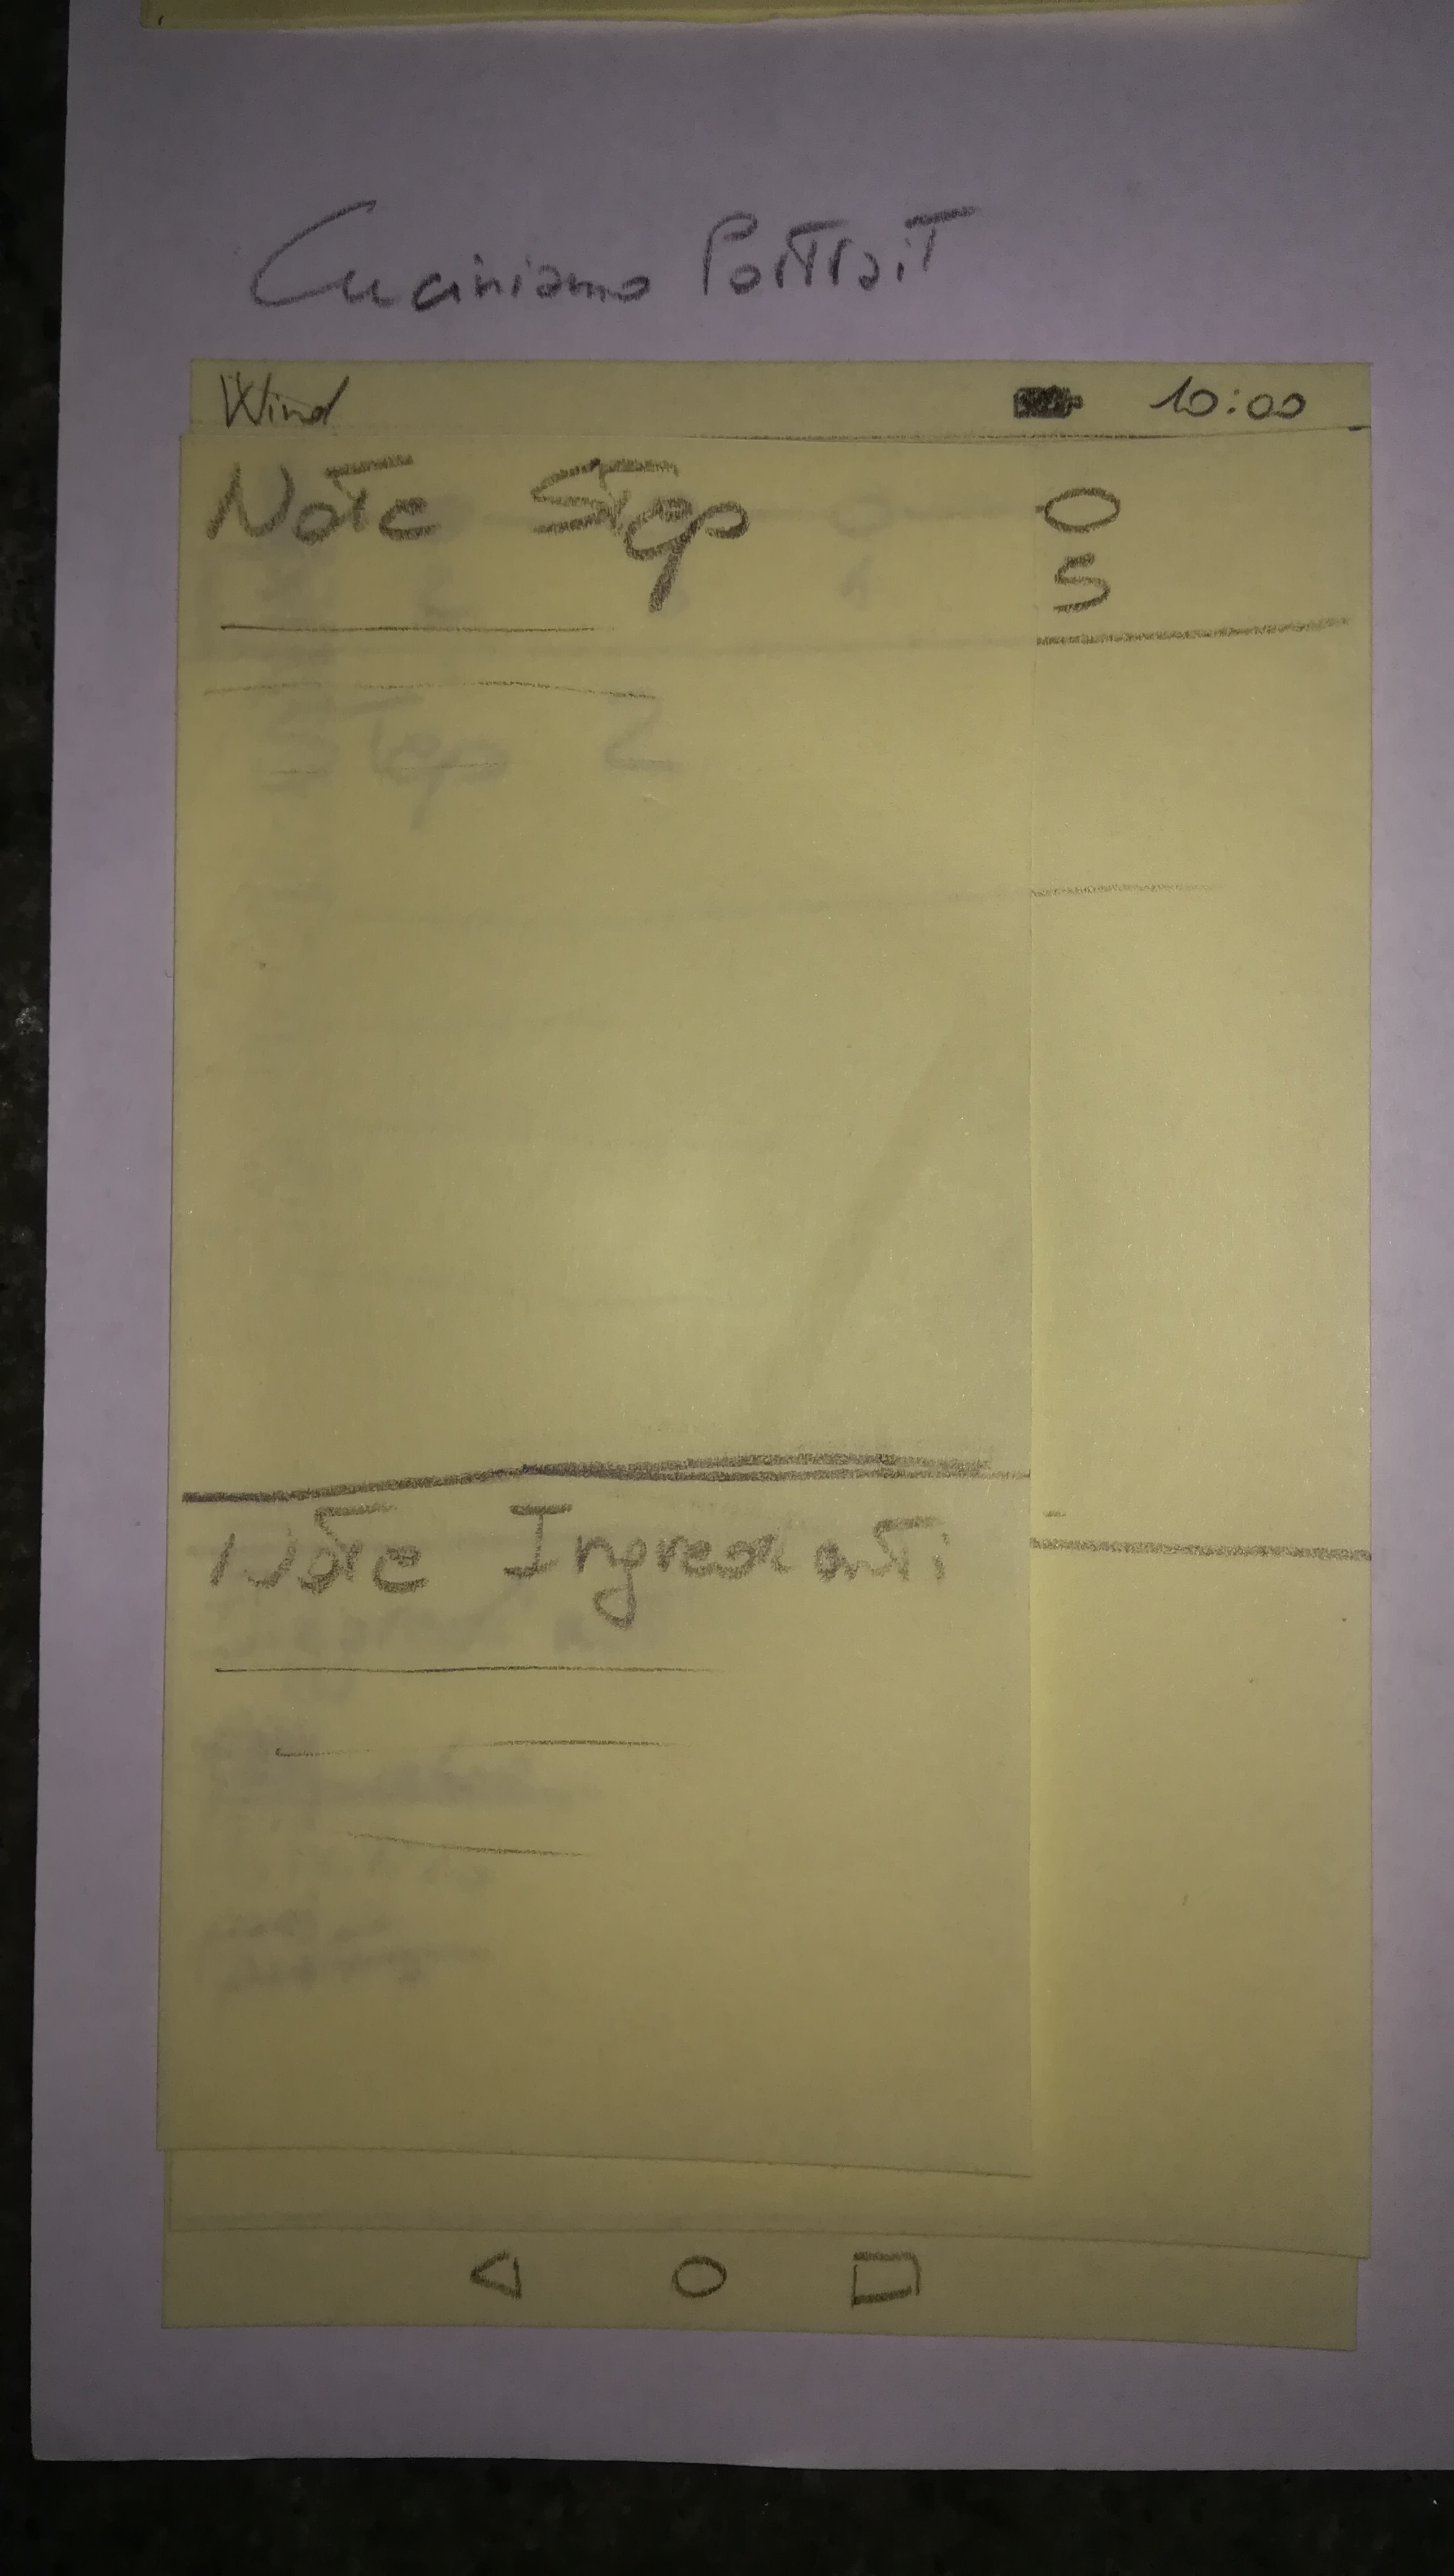
\includegraphics[width=0.4\textwidth]{prototipo2/cuciniamo_tab}
    \caption{Da sinistra a destra: riepilogo, ingredienti, preparazione}
    \label{fig:p2_cuciniamo}
  \end{center}
\end{figure}

\subsubsection{Valutazione}











\subsubsection{Design Alternativi}

\subsection{Conclusioni e Design Finale}
